\setcounter{chapter}{10}

\chapter{曲线积分与曲面积分}

曲线与曲面积分也就是在曲线和曲面上进行的积分,按照积分“分割取近似,做和求极限”的方式,
我们可以给出其精确的数学定义。从计算的角度,曲线与曲面积分与重积分一样,都可以看成是
定积分的应用。

\section{第一型的曲线积分与曲面积分}

\subsection{对弧长(第一型)的曲线积分}

% \subsubsection{【曲线的长度】}

{\bf 例:}求以下曲线的长度
\begin{enumerate}[(1)]
  \setlength{\itemindent}{1cm}
  \item $y=x^2,\;(0\leq x\leq 1)$
  \item $y=\ln\cos x,\;(0\leq x\leq\pi4)$
  \item $x^2+y^2=2x$
  \item $\rho=\cos\theta,\;(\theta\in[0,2\pi])$
\end{enumerate}

弧长的微元称为{\it 弧微分},记为$\d s$。为了便于计算,需要将其表示为与曲线
参数(曲线方程的自变量)相关的形式。
	
\begin{center}
	\resizebox{!}{5cm}{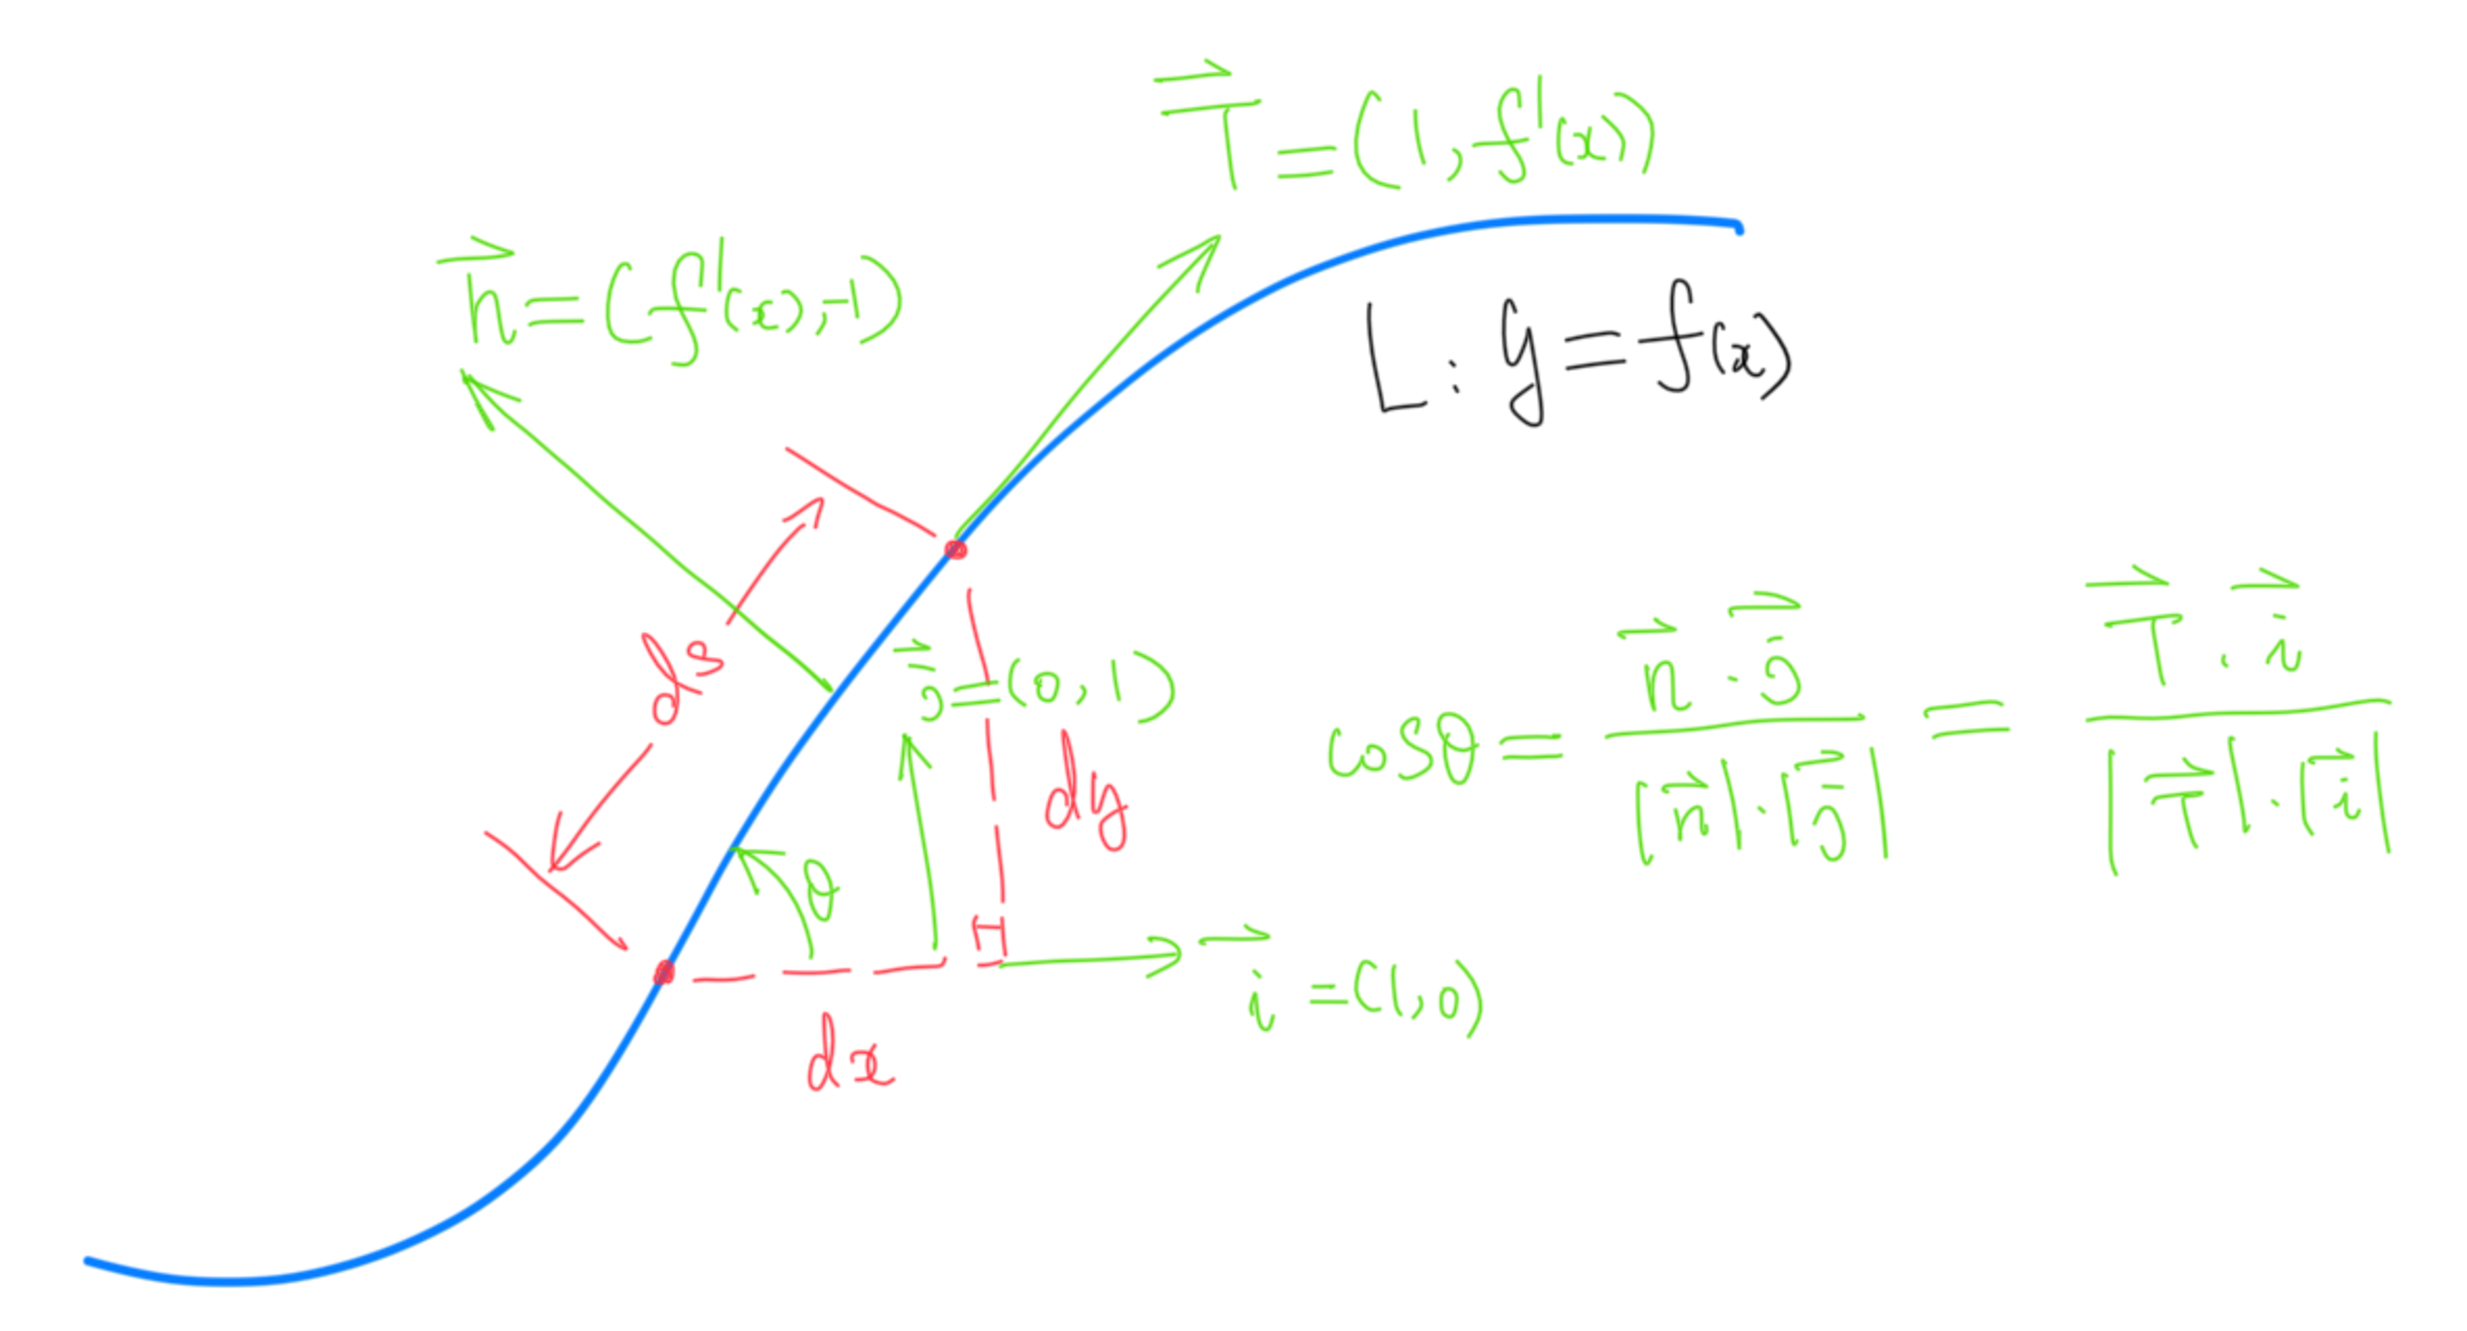
\includegraphics{./images/ch12/dsxy.pdf}}
\end{center}

如图,在曲线$L:y=f(x)$上任一点$(x,f(x))$处的一段弧长微元$\d s$,可以近似地看作是一段直线,
其在$x$和$y$上的分量分别可表示为$\d x$和$\d y$。若函数$f(x)$可微,则
$\d y=f'_x\d x$,于是
$$\d s=\sqrt{(\d x)^2+(\d y)^2}=\sqrt{1+(f'_x)^2}\d x.$$

对平面曲线,上式也可以通过另一种方式推导出来。注意到$\d x$是$\d s$在$x$轴方向上的投影,故有
$$\d x=|\cos\theta|\d s.$$
其中$\theta$为曲线的切向量$\bm{T}$与$x$轴的方向向量的夹角
(等于曲线的法向量$\bm{n}$与$x$轴法向量的夹角),也即
$$\cos\theta=\df{\bm{T}\cdot\bm{i}}{|\bm{T}||\bm{i}|}
=\df{-1}{\sqrt{1+(f'_x)^2}},$$
从而
$$\d s=\df{\d x}{|\cos\theta|}=\sqrt{1+(f'_x)^2}\d x.$$

\begin{thx}
	{\bf 平面曲线常用的弧微分公式:}分别对应于曲线的平面直角方程、参数方程和极坐标方程表示,有
	$$\d s=\sqrt{1+(y'_x)^2}\d x=\sqrt{(x'_t)^2+(y'_t)^2}\d t
	=\sqrt{(\rho'_{\theta})^2+\rho^2}\d\theta$$
\end{thx}

对弧微分(弧长微元)积分(求和)即得{\it 曲线长度},记为
$$s=\dint_L\d s$$

对于三维空间中的曲线,可以类似地推导出相应的弧微分公式。
设$L:\bm{r}(t)=(x(t),y(t),z(t)),\;(a\leq t\leq b)$, 则
$${\d s=\sqrt{(\d x)^2+(\d y)^2+(\d z)^2}
=\sqrt{(x'_t)^2+(y'_t)^2+(z'_t)^2}\d t} =|\bm{r}'(t)|\d t$$
从而曲线长度
$${s=\dint_L\d s =\dint_a^b\sqrt{(x'_t)^2+(y'_t)^2+(z'_t)^2}\d t
 =\dint_a^b|\bm{r}'(t)|\d t}$$
 
 {\bf 例:}计算圆柱螺旋线$x=\cos t,y=\sin t,z=t,(0\leq t\leq 2\pi)$的长度。

\begin{thx}
	{\bf 对弧长(第一型)的曲线积分}
	$$\dint_Lf(x,y,z)\d s,$$
	若{\it 积分路径}$L$是封闭的,上式可记为
	$$\oint_Lf(x,y,z)\d s$$
\end{thx}

{\bf 例:}已知空间曲线$L:\bm{r}(t)=(x(t),y(t),z(t)),\;(a\leq t\leq b)$,其上
的线密度为$\mu(x,y,z)$,求:
\begin{enumerate}[(1)]
  \setlength{\itemindent}{1cm}
  \item 曲线的{\it 质量}
  \item 曲线的{\it 质心}
  \item 关于$z$轴的{\it 转动惯量}
  \item 对位于$(a,b,c)$质量为$m$的质点的{\it 万有引力}
\end{enumerate}

与此前计算重积分类似,计算对弧长的曲线积分,也需要首先将其转化为定积分:
\begin{thx}
	{\bf 计算对弧长的曲线积分:}设曲线$L$可表示为$\bm{r}(t),\;(a\leq t\leq b)$,则
	$$I=\dint_Lf(\bm{x})\d s=\dint_a^bf(\bm{r}(t))|\bm{r}'(t)|\d t,$$
\end{thx}
以上的计算过程可以概括为:画图$\to$曲线参数化\ps{曲线参数化相当于对曲线进行投影,
从而确定其数学表示与参数的变化范围!}$\to$改写为定积分$\to$计算积分。特别要注意的是:
{\color{red} 将对弧长的曲线积分化为定积分时,必须保证定积分上限总是大于下限!}

对弧长的曲线积分与定积分有着非常相似的性质:
\begin{enumerate}
  \setlength{\itemindent}{1cm}
  \item {\it 线性性} 
%   \item {\it 无向性:}对弧长(第一型)的曲线积分不考虑曲线的方向,可表示为:
%   $$\dint_Lf(x,y,z)\d s=\dint_{L^-}f(x,y,z)\d s$$
  \item {\it 路径可加性:}
  $\dint_{L_1+L_2}f(x,y,z)\d s=\left(\dint_{L_1}+\dint_{
  L_2}\right)f(x,y,z)\d s$
  \item {\it 保号性}
  \item {\it 积分中值定理}
\end{enumerate}

\begin{shaded}

{\bf 关于对弧长(第一型)的曲线积分的无向性}

所谓对弧长(第一型)的曲线积分是无向的,是指其计算结果与曲线方程
中的因变量无关,也即{\it 无论选择什么样的变量作为曲线方程的参数,该参数的增大方向
是怎样的,积分的结果均相同}——{定积分也是!}——本质上,任何积分都是与积分变量无关的!

可以从两个不同的角度来理解这一点:

第一是从应用的角度,对弧长(第一型)的曲线积分可用于计算曲线的长度、质量、转动惯量、
对质点的外有引力等,这些量本身都与曲线方向无关的;

第二是从数学运算的角度,不论参数的增大方向如何,对弧长的曲线积分的结果不变。

考虑对弧长的曲线积分:
$$I=\dint_Lf(\bm{x})\d s,$$
其中曲线$L$可以表示为向量值函数
$$\bm{r}_1(t)\quad(a\leq t\leq b),$$
显然,若令$u=-t$,且记$\bm{r}_2(u)=\bm{r}_1(-u)$,
则可得$L$的另一个向量值函数表示
$$\bm{r}_2(u)\quad(-b\leq u\leq -a).$$
这两种表示最大的区别是,其中参数增大的方向是相反的。

按照以上两种方式分别计算$I$(分别记为$I_t$和$I_u$),可得
\begin{align*}
	I_u&=\dint_{-b}^{-a}f(\bm{r}_2(u))|\bm{r}'_2(u)|\d u
	=\dint_{-b}^{-a}f(\bm{r}_1(-u))|-\bm{r}'_1(-u)|\d u\\
	&=\dint_{-b}^{-a}f(\bm{r}_1(-u))|\bm{r}'_1(-u)|\d u
	=-\dint_{b}^{a}f(\bm{r}_1(t))|\bm{r}'_1(t)|\d t\\
	&=\dint_{a}^{b}f(\bm{r}_1(t))|\bm{r}'_1(t)|\d t=I_t
\end{align*}

\end{shaded}


{\bf 例:}设有点$A(1,1,0)$和$B(1,1,1)$,$L$为线段$OA,AB$和$BO$组成的封闭曲线,
方向为$O\to A\to B\to O$,计算曲线积分
$$\oint_L(x+y+z)\d s.$$

{\bf 课堂练习:}计算如下积分
$$
	\iint\limits_{x^2+y^2\leq 1}(x+y)^2\d\sigma
	\quad
	\oint_{x^2+y^2=1}(x+y)^2\d s
$$

\subsection{对面积(第一型)的曲面积分}

如何求空间曲面$\Sigma:\,z=f(x,y),\,(x,y)\in D$的面积?

% {\bf 例:}求空间曲面$\Sigma:z=x,(x,y)\in D$的面积,其中:
% \begin{enumerate}[(1)]
%   \setlength{\itemindent}{1cm}
%   \item $D:\,0\leq x\leq 1,\,0\leq y\leq 1$
%   \item $D:\,x^2+y^2\leq 1$
% \end{enumerate}
% \begin{center}
% 	\resizebox{!}{4cm}{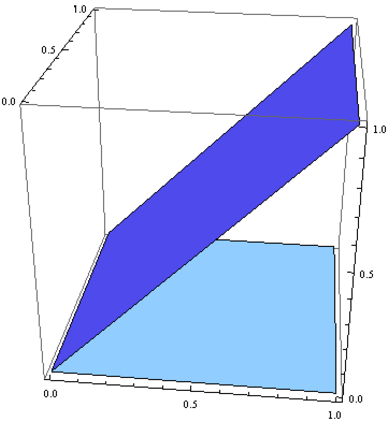
\includegraphics{./images/ch12/ssquare.pdf}}
% 	\hspace{3cm}
% 	\resizebox{!}{4cm}{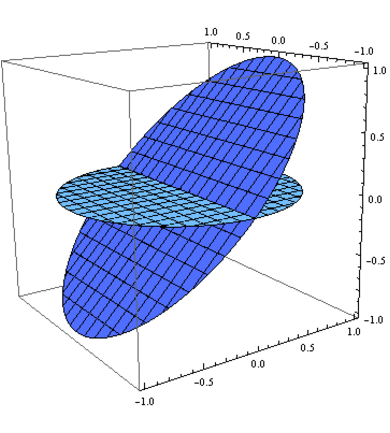
\includegraphics{./images/ch12/scircle.pdf}}
% \end{center}

\begin{thx}
	{\bf 对面积的曲面积分:}
	$$\iint_{\Sigma}f(x,y,z)\d S,$$
	其中$\Sigma$为空间曲面。若$\Sigma$是封闭的,以上积分也可以表示为
	$$\oiint_{\Sigma}f(x,y,z)\d S.$$
\end{thx}

{\bf 例:}推导球表面积公式。

\begin{thx}
	{\bf 计算对面积的曲面积分:}设曲面$\Sigma$的方程为$z=z(x,y),(x,y)\in D_{xy}$,则
	$$\iint_{\Sigma}f(x,y,z)\d S
	=\iint_{D_{xy}}f(x,y,z(x,y))\sqrt{1+(z'_x)^2+(z'_y)^2}\d\sigma_{xy}.$$
\end{thx}
和第一型的曲线积分类似,第一型的曲面积分的计算过程通过也是:画图$\to$曲面参数化(给出曲面方程)
$\to$改写为二重积分$\to$计算积分。注意到二重积分再化为累次积分时,默认也要求了上限大于下限,
因此可以说第一型的曲线和曲面积分在各方面都是非常相似的。也正因为如此,二者在基本的性质及应用方面
也是非常相似的,在此不再重复。

{\bf 例:}设空间曲面$\Sigma:\,z=f(x,y),\,(x,y)\in D$的面密度函数为
$f(x,y,z)$,求其质量。
$${M=\iint\limits_{\Sigma}f(x,y,z)\d S}$$

{\bf 例:}计算曲面积分
$$I=\oiint\limits_{\Sigma}x^2\d S,$$
其中$\Sigma$为$x+y+z=1$和坐标平面所围立体的表面。

{\bf 例:}计算曲面积分
$$\iint\limits_{\Sigma}z\d S,$$
其中$\Sigma$为柱面$x^2+y^2=1$夹在平面$z=0$和$z=1+x$之间
的部分。

{\bf 例:}设函数$y=f(x)$在区间$[a,b]$上连续可导、非负,
证明:曲线$L:\,y=f(x),x\in[a,b]$绕$x$轴旋转所得 曲面侧面积
$$S=2\pi\dint_Lf(x)\d s$$

{\bf 例:}设半球壳$z=\sqrt{R^2-x^2-y^2}$的密度为常数$\mu$,求:
\begin{enumerate}[(1)]
  \setlength{\itemindent}{1cm}
  \item 半球壳的质心;
  \item 半球壳关于$z$轴的转动惯量。
\end{enumerate}

{\bf 例:}求上半球面$z=\sqrt{1-x^2-y^2}$被$x^2+y^2=x$所截取的部分的面积与形心。

[提示]:面积$\pi-2$,形心$\left(\df{2}{3(\pi-2)},0,\df{\pi}{4(\pi-2)}\right)$

{\bf 例:}$\ds\iint_{z=\sqrt{a^2-x^2-y^2}}(x+y+z)\d S=\pi a^3$

[提示]:利用对称性化简积分。

\begin{ext}
	{\bf 课后作业}
	\begin{enumerate}
	  \item 已知$a>0$,计算积分$\dint_L z\d s$,其中$L$为$x^2+y^2=z^2$与$y^2=ax$
	  的交线上从原点到$(a,a,\sqrt2a)$的一段。
	  \item 已知$a>0$,计算积分$\dint_{\Gamma}(x^2+y^2+z^2)\d s$,其中$\Gamma$
	  为$x^2+y^2=a^2$与$z=1$的交线。
	  \item 已知某曲线$L$的线密度为$\mu=x^2+y^2+z^2$,方程为
	  $$x=e^t\cos\theta,\;y=e^t\sin\theta,\;z=\sqrt2e^t,\;-\infty<t\leq0.$$
	  求该曲线绕$z$轴转动的转动惯量。
	  \item 计算积分$\ds\iint_{\Sigma}(x+y+z)\d S$,其中$\Sigma$为半径为
	  $R$的上半球面。
	  \item 计算积分$\ds\iint_S x^2\d S$,其中$S$为圆柱面$x^2+y^2=a^2$介于
	  $z=0$和$z=h$之间的部分。
	  \item 计算积分$\ds\iint_{\Sigma}(ax^2+by^2+cz^2)\d S$,其中
	  $\Sigma$为单位球面。
	  \item 设球面$x^2+y^2+z^2=2x$的面密度$\mu=x^2+y^2+z^2$,求其质量。
	\end{enumerate}
\end{ext}

\section{对坐标(第二型)的曲线积分}

{\bf 例:}已知某质点$M$在{\it 引力场}
$$\bm{F}(x,y,z)=(P(x,y,z),Q(x,y,z),R(x,y,z))$$
中沿曲线$L:\bm{r}(t)=(x(t),y(t),z(t)),(a\leq t\leq b)$
运动,求引力对其做的功。

\begin{thx}
	{\bf 对坐标(第二型)的曲线积分:}
	$${W=\dint_L\bm{F}\d\bm{s}=\dint_LP\d x+\dint_LQ\d y+\dint_LR\d z}$$
	其中,若$L$为封闭曲线,则可记为:
	$$W=\oint_LP\d x+Q\d y+R\d z$$
\end{thx}

设曲线$L$可表示为$\bm{r}(t),\;(a\leq t\leq b)$,则
\begin{thx}
	$$I=\dint_L\bm{F}(\bm{x})\d\bm{s}
	=\dint_a^b\bm{F}(\bm{r}(t))\cdot\bm{r}'(t)\d t,$$
\end{thx}
{\b 在上式右端的定积分中,必须确保下限对应曲线起点,上限对应曲线终点!}
\begin{enumerate}[(1)]
  \setlength{\itemindent}{1cm}
  \item {\it 有向性:}
  $$\dint_LP\d x+Q\d y+R\d z=-\dint_{L^-}P\d x+Q\d y+R\d z$$
  \item {\it 路径可加性:} 设$L=\bigcup_{k=1}^nL_k$, 且$L$与$L_k(k=1,2,\ldots,n)$
  方向均一致, 则
  $$\dint_LP\d x+Q\d y+R\d z=\sum\limits_{k=1}^n\dint_{L_k}P\d x+Q\d y+R\d z$$
\end{enumerate}

{\bf 注:}由对坐标(第二型)曲线积分的有向性和路径可加性,可导出如下有趣的性质。如图:
\begin{center}
	\resizebox{!}{5cm}{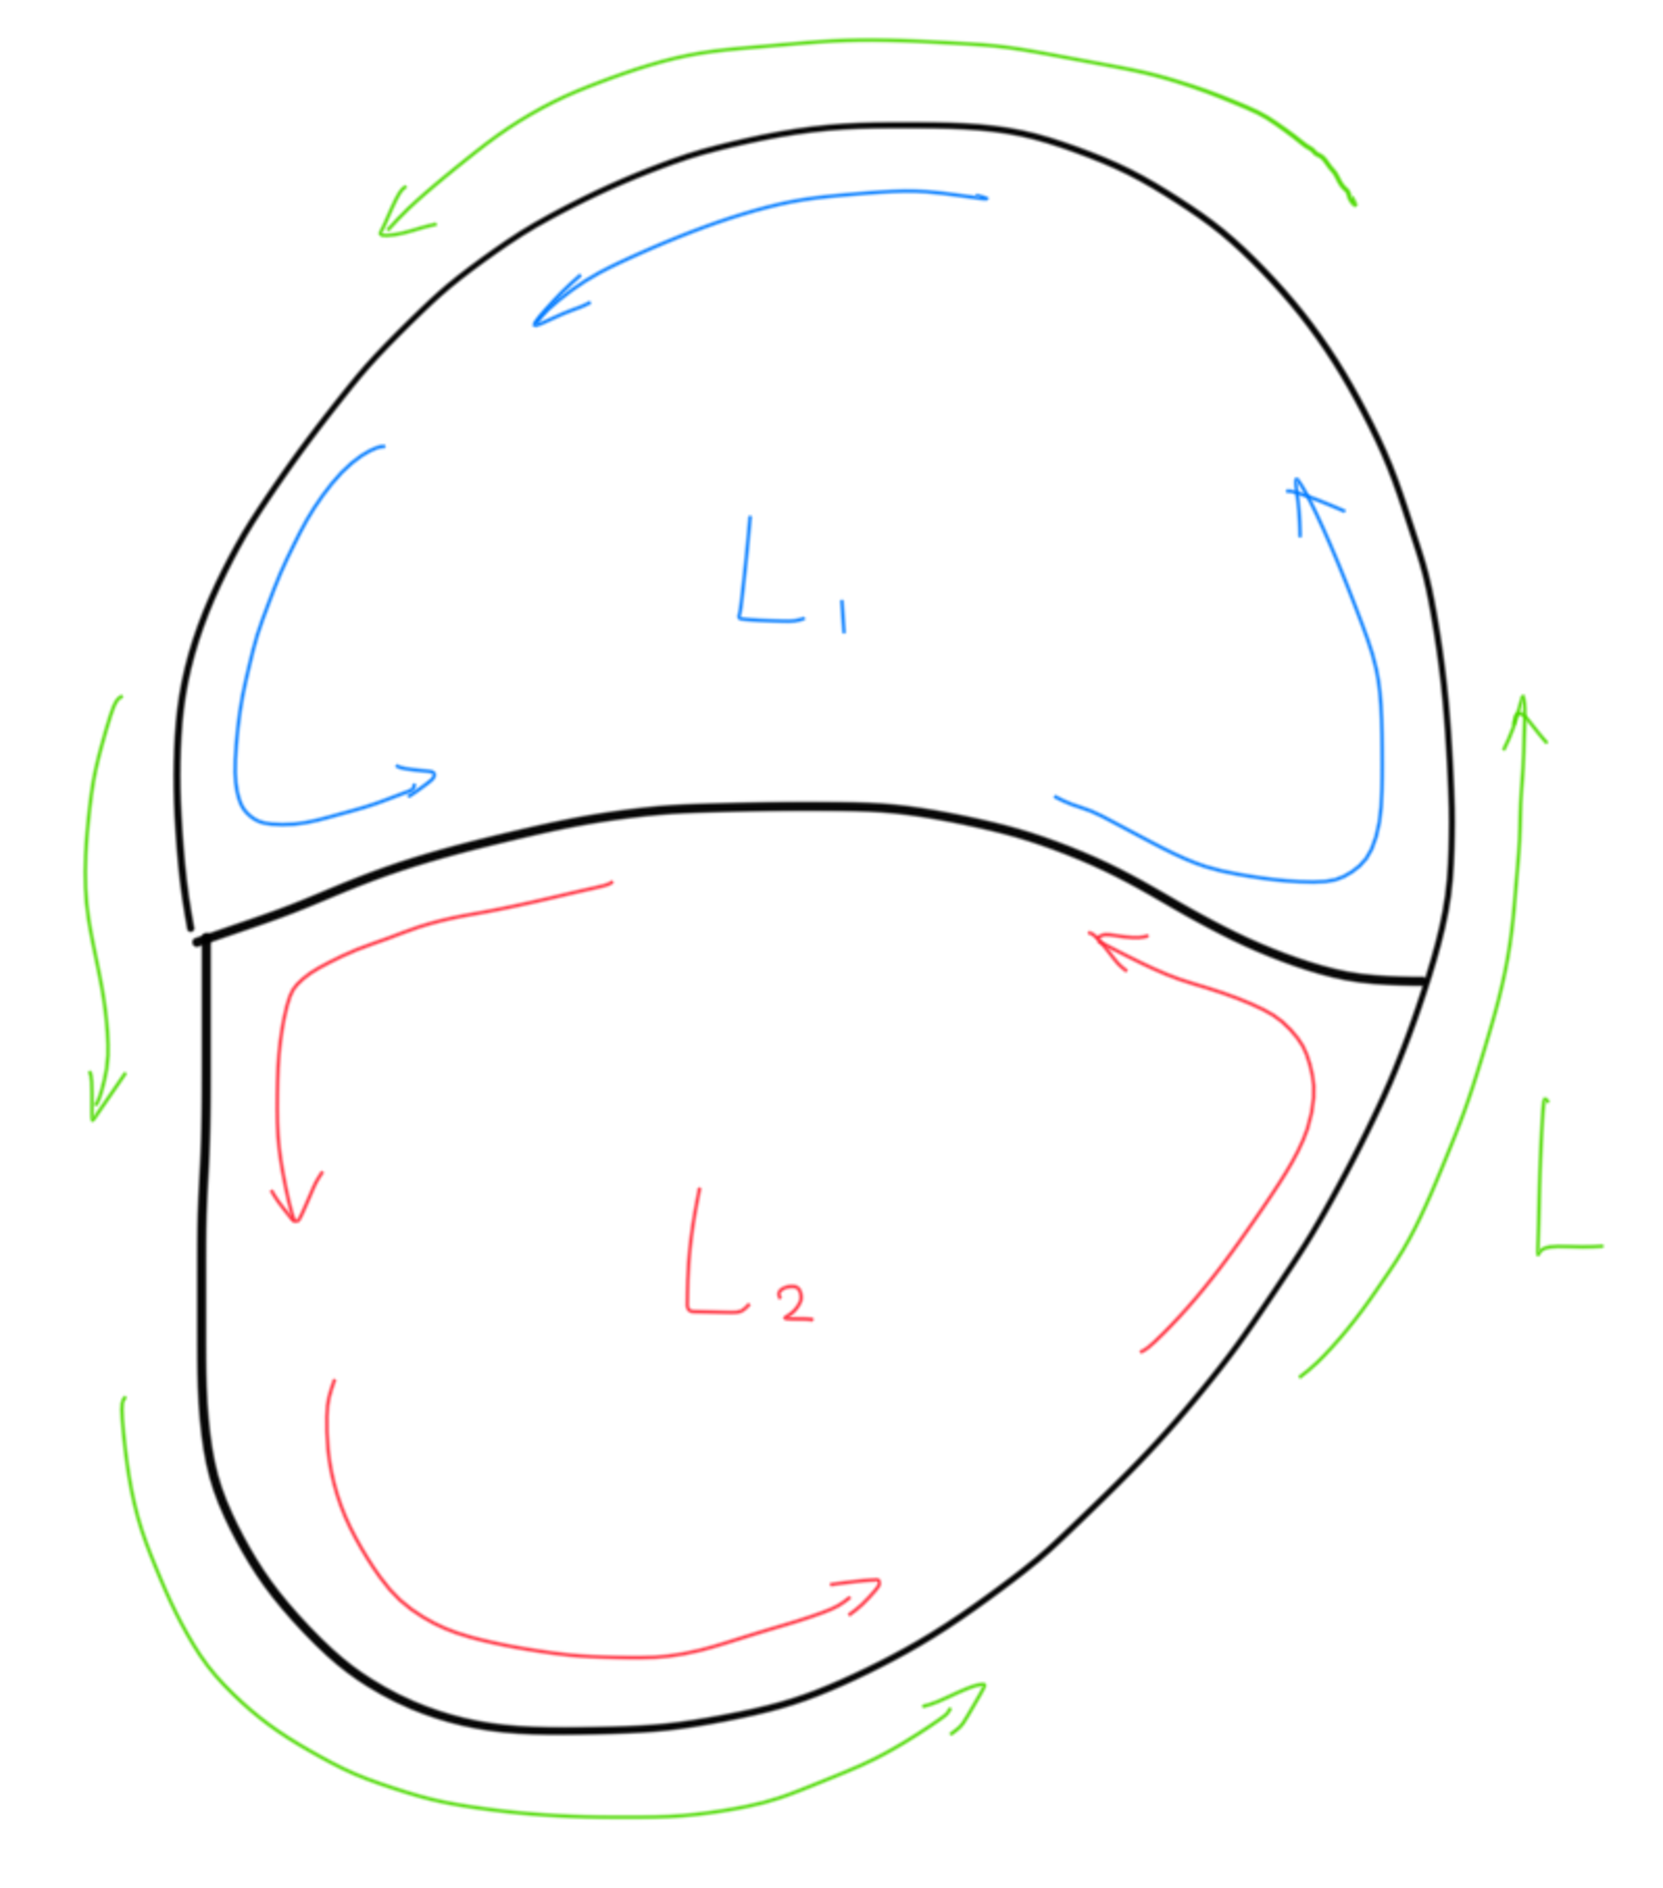
\includegraphics{./images/ch12/2ndCI.pdf}}
\end{center}
$$\oint_{L}\bm{f}(\bm{x})\d\bm{s}
=\left(\oint_{L_1}+\oint_{L_2}\right)\bm{f}(\bm{x})\d\bm{s}$$

% \subsubsection{【计算】}

{\bf 例:}设有点$A(1,1,0)$和$B(1,1,1)$,$L$为线段$OA,AB$和$BO$组成的封闭曲线,
方向为$O\to A\to B\to O$,分别计算曲线积分
$$\oint_L(x+y+z)\d s\quad\mbox{和}\quad\oint_Lx\d x+y\d y+z\d z.$$

{\bf 注:}对坐标(第二型)的曲线积分的计算步骤:
画图$\to$曲线参数化$\to$定限$\to$积分

\subsection{两类曲线积分的关系}

\begin{thx}
	{\bf 对坐标的曲线积分总可以化为对弧长的曲线积分:}
	设$L:\bm{r}(t)=(x(t),y(t),z(t)),\;(a\leq t\leq b)$, 其单位切向量
	$$\bm{T}=\pm\df{\bm{r}'(t)}{|\bm{r}'(t)|},$$
	({\color{red}$\bm{T}$指向$L$的正向,若其与$t$的正向(增大方向)一致,则
	取正号,否则取负号}),进而可得
	$$\dint_L\bm{F}\cdot \d\bm{s}=\dint_L\bm{F}\cdot\bm{T}\d s
	=\pm\dint_L\bm{F}\cdot\bm{r}'(t)\d t$$
\end{thx}
事实上,利用以上的公式,也可以将对弧长的曲线积分总可以化为对坐标的曲线积分。
 
{\bf 例:}计算曲线积分$\dint_Lxy\d x$,其中积分曲线$L$分别为:
\begin{enumerate}[(1)]
  \setlength{\itemindent}{1cm}
  \item 由原点沿$y=x^3$至$A(1,1)$;
  \item 由原点沿$y^2=x$至$A(1,1)$。
\end{enumerate}

{\bf 例:}计算曲线积分$\dint_Ly\d x-x\d y$,其中积分曲线$L$分别为:
\begin{enumerate}[(1)]
  \setlength{\itemindent}{1cm}
  \item 由$A(0,-1)$沿右半单位圆至$B(0,1)$;
  \item 由$A(0,-1)$沿左半单位圆至$B(0,1)$;
  \item 由$A(0,-1)$沿单位圆逆时针方向至$A(0,-1)$。
\end{enumerate}

% \subsection{曲线积分的应用}
% 
% \begin{enumerate}
%   \item {\bf 对弧长的曲线积分:}
%   \begin{itemize}
%     \item 曲线的长度、质量
%     \item 曲线的质心、转动惯量
%     \item 曲线对质点的引力
%   \end{itemize}
%   \item {\bf 对坐标的曲线积分:}
%   \begin{itemize}
%     \item 变力沿曲线做功
%     \item {向量场中的环量和流量}
%   \end{itemize}
% \end{enumerate}

\subsection{流量与环量}

考虑平面区域内$D$内的向量场
$$\bm{v}=(P(x,y),Q(x,y)),\;(x,y)\in D.$$
$L:\bm{r}=\bm{r}(t)$为$D$内简单光滑闭曲线,取逆时针方向。
$\bm{T},\bm{n}$分别为$L$的单位切向量和单位法向量。

{\bf 约定:}{\b 以上切向量$\bm{T}$的方向为路径$L$的方向,法向量$\bm{n}$默认为
$\bm{T}$的右侧\ps{KD教材上所谓“外侧”法向量的
说法是不准确的!}(顺时针旋转$\pi/2$所得)法向量。}\ps{顺时针旋转矩阵:
$$\left[\begin{array}{cc}
	\cos\theta & \sin\theta \\ -\sin\theta & \cos\theta
\end{array}\right]$$
}因此,由
$$\bm{T}\cdot\d\bm{s}=(\d x, \d y)\quad\Rightarrow
\quad\bm{n}\cdot\d\bm{s}=(\d y,-\d x)$$

\begin{itemize}
  \item {\it 流量:}$\ds\oint_L\bm{v}\cdot\bm{n}\d s=\oint_LP\d y-Q\d x$
  {\;—“向量场穿过$L$的总流速”}
  \item {\it 环量:}$\ds\oint_L\bm{v}\cdot\bm{T}\d s=\oint_LP\d x+Q\d y$
  {\;—“向量场环绕$L$的总流速”}
\end{itemize}

\begin{center}
	\resizebox{!}{5cm}{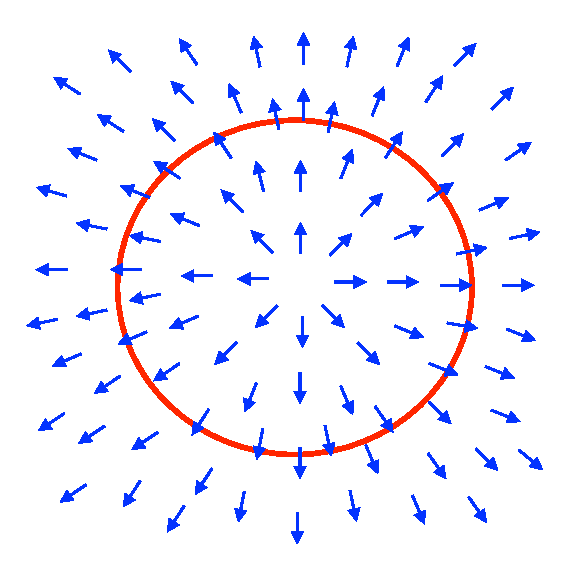
\includegraphics{./images/ch12/flow.pdf}}\hspace{2cm}
	\resizebox{!}{5cm}{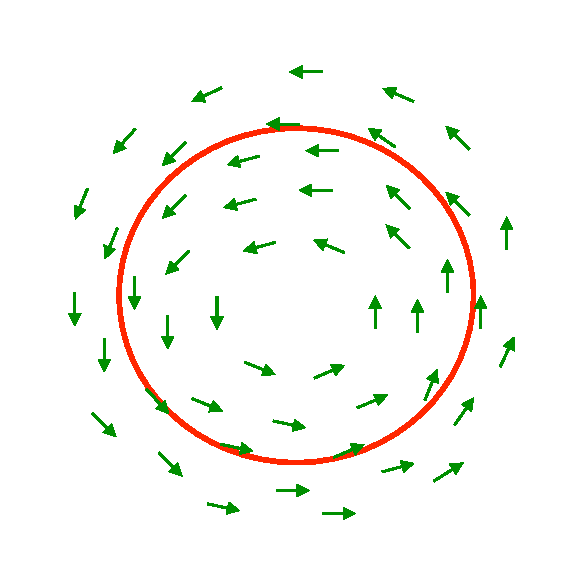
\includegraphics{./images/ch12/rotate.pdf}}
	
	{\it 流量:}${\ds\oint_L\bm{v}\cdot\bm{n}\d s}$\hspace{4cm}
	{\it 环量:}${\ds\oint_L\bm{v}\cdot\bm{T}\d s}$
\end{center}

{\bf 例:}设$L$为平面上的简单光滑闭曲线,$D$为$L$所围成的有界闭区域,$\bm{n}$
为$L$的外法向,$\df{\p u}{\p\bm{n}}$表示函数$u(x,y)$沿$\bm{n}$的方向导数
\begin{enumerate}[(1)]
  \item 将$\ds\oint_L\df{\p u}{\p\bm{n}}\d s$化为对坐标的曲线积分;
  \item 设$u=x^2+y^2$,$L:x^2+y^2=6x$,计算
  $$\ds\oint_L\df{\p u}{\p\bm{n}}\d s$$
\end{enumerate}

{\bf 例:}分别计算向量场
$$\bm{v}_1=(x,y)\quad\mbox{和}\quad \bm{v}_2=(-y,x)$$
沿单位圆逆时针方向的流量和环量。

\begin{ext}
	{\bf 课后作业}
	\begin{enumerate}
	  \item 设$L$为曲线$x=\df{3at}{1+t^3},y=\df{3at^2}{1+t^3}$上$t$由
	  $0$到$+\infty$的一段,$a>0$,计算$\dint_Lx\d y-y\d x$。
	  \item 计算积分
		$$I=\int_Ly^2\d x+z^2\d y+x^2\d z,$$
		其中$C$为曲线$\left\{\begin{array}{l}
		x^2+y^2+z^2=1 \\ x^2+y^2=x
		\end{array}\right.$
		上$z\geq 0$的部分,从$x$轴正向看去为逆时针方向。
% 	  \item 设$L$为平面上的简单光滑闭曲线,$D$为$L$所围成的有界闭区域,$\bm{n}$
% 		为$L$的外法向,$\df{\p u}{\p\bm{n}}$表示函数$u(x,y)$沿$\bm{n}$的方向导数
% 		\begin{enumerate}[(1)]
% 		  \item 将$\ds\oint_L\df{\p u}{\p\bm{n}}\d s$化为对坐标的曲线积分;
% 		  \item 设$u=x^2+y^2$,$L:x^2+y^2=6x$,计算
% 		  $\ds\oint_L\df{\p u}{\p\bm{n}}\d s$。
% 		\end{enumerate}
	\end{enumerate}
\end{ext}

\section{Green公式与保守场}

\subsection{Green公式}

\begin{thx}
	{\bf Green公式:}
	$$\oint_LP(x,y)\d x+Q(x,y)\d y=\iint_D\left(
	\df{\p Q}{\p x}-\df{\p P}{\p y}\right)\d\sigma_{xy}$$
	其中:
	\begin{itemize}
	  \item $D$为$xOy$平面内的有界闭区域
	  \item $L=\p D$:分段光滑曲线,按{\it “左侧法则”}取正向
	  \item $P(x,y),Q(x,y)$在$D$内有连续偏导数
	\end{itemize}
\end{thx}

{\bf 例:}沿单位圆的逆时针方向计算以下曲线积分
$$\oint_Lx\d x+y\d y,\hspace{3em}\oint_Ly\d x+x\d y$$

{\bf 注:}使用Green公式需要注意以下几点:
\begin{enumerate}[(1)]
  \setlength{\itemindent}{1cm}
  \item {\it 左侧法则:}积分区域始终位于曲线方向的左侧;
  \item 区域$D$必须有界;
  \item $D$的边界可以包含平行于$x$轴和$y$轴的直线;
  \item $D$可以是简单闭区域、单连通域和多连通域;
\end{enumerate}

{\bf 例:}计算椭圆$\df{x^2}{a^2}+\df{y^2}{b^2}\leq 1\,(a>0,b>0)$的面积。

$$\oint_L x\d y-y\d x=2\iint_D\d\sigma$$

{\bf 例:}曲线$C$为右半单位圆沿$(0,1)$至$(0,-1)$的路径,求
$$\int_C(\cos x+y)\d x+(x+\sin y)\d y.$$

{\bf 注:}对于非封闭路径上的第二型曲线积分,必须补全路径后才能使用Green公式!

{\bf 例:}设$L$是摆线$x=t-\sin t-\pi,y=1-\cos t$从$t=0$
到$t=2\pi$的一段,则$\dint_L\df{(x-y)\d x+(x+y)\d y}{x^2+y^2}=-\pi$

[提示]:添加路径$L_1:x^2+y^2=\pi^2,\;y\geq 0$,使用Green公式计算。
注意,不能使用路径$y=0$,因为被积函数在原点处无定义!

{\bf 例:}设有流速场
$$\bm{v}(x,y)=\left(\df{x}{x^2+y^2},
\df{y}{x^2+y^2}\right),\;(x^2+y^2\ne 0),$$
求其通过以下闭曲线(均取逆时针方向)的流量:\ps{{\b 本题须重点掌握!}
理解为何要“挖洞”?如何“挖洞”?
“挖洞”后如何计算所求的积分?}
\begin{enumerate}[(1)]
  \setlength{\itemindent}{1cm}
  \item $L_1$:不经过原点且不包含原点的任一光滑闭曲线;
  \item $L_2$:$x^2+y^2=R^2$
  \item $L_3$:$\df{x^2}{a^2}+\df{y^2}{b^2}=1\,(a>0,b>0)$
\end{enumerate}

\begin{shaded}
	{\bf 关于“挖洞”问题}
	
	“挖”什么形状的“洞”需要根据题目的特点来决定,例如下面的例子,“挖”
	一个圆形的“洞”,就不如“挖”一个椭圆形的“洞”
	
	{\it\b NUDT的命题习惯:第一型曲线(曲面)积分一般考直接计算,
	第二型曲线积分常考Green公式的使用,特别是“挖洞”,第二型曲面积分常考Gauss公式
	的使用,特别是“补全”}
	
	{\bf NUDT-2015春}:已知$C$为不经过原点的简单光滑闭曲线,取逆时针方向为正向,
	$a>b>0$,计算曲线积分
	$$\oint_C\df{y\d x-x\d y}{ax^2+by^2}$$
	
	[提示]:记$P=\df{y}{ax^2+by^2},Q=\df{-x}{ax^2+by^2}$,可以验证
	在原点之外均有
	$$\df{\p P}{\p y}=\df{\p Q}{\p x}.$$
	
	根据原点是否在$C$内部进行讨论。
	
	1)若原点位于$C$的外部,利用Green公式,可得结果为零;
	
	2)若原点位于$C$的内部,则在$C$内“挖洞”,洞的边界为
	$$C_{\e}:\;ax^2+by^2=\e,\quad(\e>0),$$
	进而可得在$C$上的积分,等于在$C_{\e}$上的积分,后者利用第二型曲线
	积分的计算公式计算,结果为$-\df{2\pi}{\sqrt{ab}}$。
	
	{\bf NUDT-2016春}:已知$C$为不经过原点的简单光滑闭曲线,取逆时针方向,
	计算曲线积分
	$$\oint_C\df{(x+y)\d x-(x-y)\d y}{(x^2+y^2)}$$
	
	[提示]:常规的“挖洞”问题,若原点不在$C$内,结果为零;若在$C$内,结果为$-3\pi$.
	
	{\bf NUDT-2012春}:计算曲线积分
	$$\oint_L\left(x-\df{y}{x^2+y^2}\right)\d x
	+\left(y+\df{x}{x^2+y^2}\right)\d y,$$
	其中$L:\df{x^2}9+\df{y^2}4=1$为逆时针方向。
	
	[提示]:利用“挖洞”简化计算,结果为$2\pi$。根据被积函数的特点,所挖“洞”
	的形状应为圆形。
	
	{\bf 例:}$L$为逆时针的单位圆,计算积分
	$$\oint_L\df{(x-y)\d x+(x+4y)\d y}
	{x^2+4y^2}$$
	
	[提示]:利用“挖洞”简化计算,根据被积函数的特点,“洞”的边界为
	$$C_{\e}:x^2+4y^2=\e^2\quad(0<\e<<1)$$
	
	{\bf 例:}计算积分
	$$I=\oint_C\df{\cos(\bm{r},\bm{n})}{r}\d s,$$
	其中$C$为不包含原点的分段光滑闭曲线,$\bm{r}=(x,y)$,$r=|\bm{r}|$,
	$\bm{n}$为$C$的外侧单位法向量
		
	[提示]:
	$$I=\oint_C\df{\bm{r}\cdot\bm{n}}{r^2}\d s
	=\oint_C\df{x\d y-y\d x}{x^2+y^2}$$
	根据原点是否在$C$内部讨论。
	原点不在$C$内时为$0$,直接使用Green公式,结果为$0$;
	原点在$C$内时,“挖洞”处理,结果为$2\pi$
	
	{\bf 命题:}{\b 若$ac-b^2>0$,则
	$\df{x\d y-y\d x}{ax^2+2bxy+cy^2}$
	为全微分。}
	
	[提示]:记$p=\df{c}{\sqrt{ac-b^2}}$,
	\begin{align*}
		\df{x\d y-y\d x}{ax^2+2bxy+cy^2}
		&=\df{\frac1x\d y-\frac y{x^2}\d x}{a+2b\frac yx+c\left(\frac yx\right)^2}
		=\df{\d\frac yx}{c\left[\frac yx-\frac bc\right]^2+\frac{ac-b^2}{c}}\\
		&=\df{\d\left(\frac yx-\frac bc\right)}{c\left[\frac yx-\frac
		bc\right]^2+\frac{ac-b^2}{c}}
		=p\df{\d p\left(\frac yx-\frac bc\right)}{\left[p\left(\frac yx-\frac
		bc\right)\right]^2+1}\\
		&=\d\left[p\arctan p\left(\df yx-\df bc\right)\right]
	\end{align*}
	
	{\bf 注:}椭圆$ax^2+2bxy+cy^2=1$的面积为$\df{\pi}{\sqrt{ac-b^2}}$
\end{shaded}

\subsection{向量场与Green公式}

\subsubsection{散度与无源场}

\begin{thx}
	已知流速场
	$$\bm{v}=(P(x,y),Q(x,y)),\;(x,y)\in D,$$
	满足Green公式条件 ,则
	$${\mathrm{div}\,\bm v=\df{\p P}{\p x}+\df{\p Q}{\p y}}$$
	称为$\bm{v}$的{\bf 散度}。若在区域$D$内$\mathrm{div}\bm{v}$处处为零,
	则称$\bm{v}$是$D$内的{\bf 无源场}。 
\end{thx}
显然,Green公式可以写成
$$\oint_L\bm{v}\cdot\bm{n}\d s=\iint_D\mathrm{div}\,\bm{v}\,\d\sigma,$$
这种形式的Green公式称为{\kaishu 散度形式的Green公式}。

\subsubsection{无旋场}

已知向量场
$$\bm{v}=(P(x,y),Q(x,y)),\;(x,y)\in D,$$
满足Green公式条件 ,则
$$\oint_L\bm{v}\cdot\bm{T}\d s=\iint\limits_D\left(
\df{\p Q}{\p x}-\df{\p P}{\p y}\right)\d\sigma,$$
该公式称为{\kaishu 旋度形式的Green公式}。
\begin{thx}
	若向量场$\bm{v}=(P,Q)$在$D$内总满足${\df{\p Q}{\p x}-\df{\p P}{\p y}=0}$,
	则称之为$D$内的{\bf 无旋场}。
\end{thx}
显然
\begin{thx}
	\begin{enumerate}%[(1)]
% 	  \setlength{\itemindent}{1cm}
	  \item 区域$D$内的向量场为无源场,则通过$\p D$的流量为$0$
	  \item 区域$D$内的向量场为无旋场,则沿$\p D$的环量为$0$
	\end{enumerate}
\end{thx}

\subsection{保守场与积分路径无关性}

设区域$D$内有向量场
$\bm{F}(x,y)=(P(x,y),Q(x,y))$,
在$D$内任取两点$A,B$,若由$A$到$B$沿任意路径所做的功都一样,
也即积分
$$\dint_{L_{AB}}P\d x+Q\d y$$
的值是与积分路径无关的,
则称$\bm{F}(x,y)$为区域$D$内的一个保守场

\begin{thx}
	{\bf 保守场与积分路径无关性:}$\bm{F}(x,y)=(P(x,y),Q(x,y))$为单连通域$D$内的向量场,
	$P,Q$具有一阶连续偏导数,则以下条件等价:
	\begin{enumerate}[(1)]
% 	  \setlength{\itemindent}{1cm}
	  \item $\bm{F}$是$D$内的保守场;
	  \item $\bm{F}$是$D$内的无旋场;
	  \item 存在$u(x,y)$,使得
	  $$\d u(x,y)=P(x,y)\d x+Q(x,y)\d y,\;(x,y)\in D$$
	\end{enumerate}
\end{thx}

{\bf 例:}$f(x)$连续可导,$L$为$(3,2/3)$到$(1,2)$的直线,
则$\dint_L\df{1+y^2f(xy)}y\d x+\df x{y^2}[y^2f(xy)-1]\d y=-4$

[提示]:积分与路径无关!

\subsection{原函数与全微分}

根据前述定理,设$\bm{F}=(P,Q)$是$D$内的保守场,则存在$u(x,y)$,使得
$$\d u(x,y)=P(x,y)\d x+Q(x,y)\d y,\;(x,y)\in D$$
 $u(x,y)$称为: 微分式$P\d x+Q\d y$的{\it 原函数},或
向量场$\bm{F}$的{\it 势函数}。

$${\dint_{L_{AB}}P\d x+Q\d y=u(x,y)|_A^B} $$
显然$u(x,y)$不唯一(不同的原函数可能相差一个常数)!

{\bf 原函数的计算——折线法:}\ps{强烈不推荐使用!!}

$\bm{F}=(P,Q)$是$D$内的保守场,求其势函数$u(x,y)$
\begin{enumerate}[Step-1:]
  \setlength{\itemindent}{1cm}
  \item 任取$A(x_0,y_0),\,B(x,y)\in D$ 
  \item 取折线
  $${L:\,A(x_0,y_0)\to C(x,y_0)\to B(x,y)} $$
  \item 计算积分
  \begin{eqnarray*}
  	u(x,y)&=&\dint_LP(x,y)\d x+Q(x,y)\d y \\
  	&=&{\dint_{x_0}^xP(x,y_0)\d x+\dint_{y_0}^yQ(x,y)\d y}
  \end{eqnarray*}
\end{enumerate}

{\bf 例:}验证向量场
$$\bm{F}=(4x^3y^3-3y^2+5,3x^4y^2-6xy-4)$$
为$xOy$平面上的保守场,并求$\bm{F}$的势函数。利用势函数计算
$\bm{F}$沿以$(0,1)$为起点,$(1,2)$为终点的路径所做的功。

{\bf 例}(NUDT-2010春)证明存在区域$D=\{(x,y)|x>0,y>0\}$
内的函数$u(x,y)$,满足
$$\d u(x,y)=\left(\df yx+\df{2x}y\right)\d x
+\left(\ln x-\df{x^2}{y^2}\right)\d y,$$
并求出满足$u(1,1)=0$的函数$u(x,y)$。

{\bf 例:}求下列全微分的原函数
\begin{enumerate}[(1)]
  \setlength{\itemindent}{1cm}
  \item $(x^2+2xy-y^2)\d x+(x^2-2xy-y^2)\d y$
  \item $e^x[e^y(x-y+2)+y]\d x+e^x[e^y(x-y)+1]\d y$
  \item $(\sqrt{x^2+y^2})x\d x+(\sqrt{x^2+y^2})y\d y$
\end{enumerate}

{\bf 例:}利用全微分法计算曲线积分
\begin{enumerate}[(1)]
  \setlength{\itemindent}{1cm}
  \item $\dint_{(1,1,1)}^{(2,3,-4)}x\d x+y^2\d y-z\d z$
  \item $\dint_{(1,1,1)}^{(2,3,-4)}(x+y+z)^3(\d x+\d y+\d z)$
\end{enumerate}

\begin{thx}
	若存在$u(x,y)$,满足:
	$$\d u(x,y)=P(x,y)\d x+Q(x,y)\d y,$$
	则称$P(x,y)\d x+Q(x,y)\d y=0$为{\bf 全微分方程}
\end{thx}

{\bf 注:}$P(x,y)\d x+Q(x,y)\d y=0$为全微分方程当且仅当
\ps{以下的条件也称为{\b Cauchy-Riemann方程/条件}}
$$\df{\p P}{\p y}=\df{\p Q}{\p x}$$

{\bf 例:}求微分方程
$$(3x^2+6xy^2)\d x+(6x^2y+4y^3)\d y=0$$
的通解。

{\bf 积分因子法求解微分方程:}

{\bf 例:}求解微分方程:$x\d y-y\d x=0$。

通过两边同时乘以特定的函数({\it 积分因子})\ps{关于如何求积分因子,是一个比较复杂的问题,
重点掌握一些常见的积分因子即可。另外,积分因子可能是不唯一的!}
,可以使原方程化为全微分方程:
$${\df 1{y^2}}(x\d y-y\d x) =-\d\left(\df xy\right)
=0,\quad {\df{1}{x^2+y^2}}(x\d y-y\d x) =-\d\arctan\df xy=0$$

\begin{ext}
	{\bf 课后作业}
	\begin{enumerate}
	  \item 已知$C$为不经过原点的简单光滑闭曲线,取逆时针方向为正向,
	  $a>b>0$,计算曲线积分$\ds\oint_C\df{y\d x-x\d y}{ax^2+by^2}$。
	  \item 设$L$是摆线$x=t-\sin t-\pi,y=1-\cos t$从$t=0$
	  到$t=2\pi$的一段,计算$\dint_L\df{(x-y)\d x+(x+y)\d y}{x^2+y^2}$。
	  \item 函数$f(r)$二阶连续可导,$r=\sqrt{x^2+y^2}$,
  	  若$\mathrm{div}(\bigtriangledown\,f(r))=0$,求$f(r)$。
  	  \item 设$f(x)$当$x>0$时可导,$f(1)=1$,对右半平面内的任意封闭曲线$C$,
	  总有$\ds\oint_C4x^3y\d x+xf(x)\d y=0$,求$f(x)$,并计算积分
	  $\dint_{(1,0)}^{(2,3)}4x^3y\d x+xf(x)\d y$。
	  \item 设$f(x,y)$处处偏导连续,积分$\dint_Lf(x,y)\d x+x\cos x\d y$
	  在全平面内与路径无关,且$\dint_{(0,0)}^{(t,t^2)}f(x,y)\d x+x\cos x\d y
	  =t^2$,求$f(x,y)$。
	\end{enumerate}
\end{ext}

\section{对坐标(第二型)的曲面积分}

{\bf 例:}已知曲面$\Sigma:\,z=f(x,y),\,(x,y)\in D$和流速场
$$\bm{v}(x,y,z)=(P(x,y,z),Q(x,y,z),R(x,y,z)),$$
求经过该曲面的流量。

{\bf 约定:}沿给定法方向流过$\Sigma$的流量为正,反之为负

\begin{shaded}
	{\bf 关于曲面方向的约定}
	\begin{itemize}
	  \setlength{\itemindent}{1cm}
	  \item {\it 双侧曲面:}
	  \begin{itemize}
	    \setlength{\itemindent}{1cm}
	    \item {\it 封闭曲面:外侧为正,内侧为负}
	    \item 开放曲面:任取一侧为正,一侧为负
	  \end{itemize}
	  \item {\it 单侧曲面:}无方向(如下图的Mobius带和Klein瓶)
	\end{itemize}
	\begin{center}
		\resizebox{!}{4.5cm}{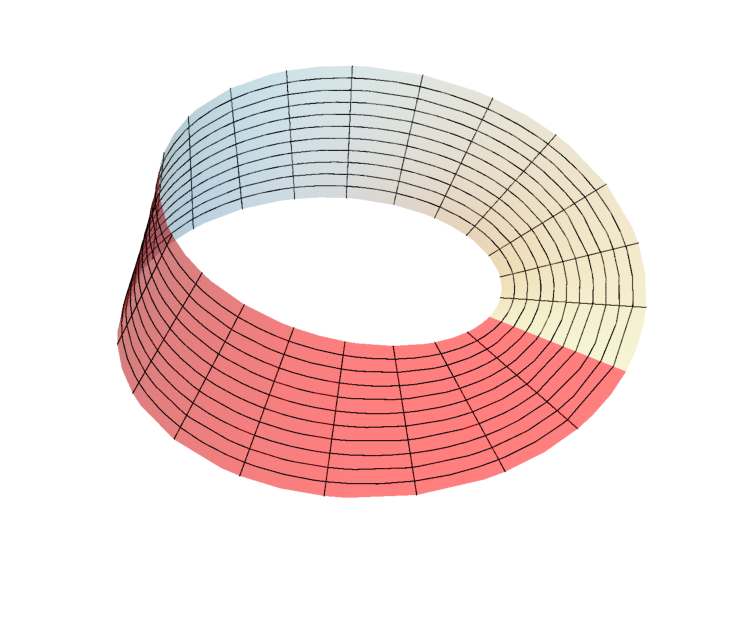
\includegraphics{./images/ch12/MobiusStrip.pdf}}
		\quad\quad\quad
		\resizebox{!}{4.5cm}{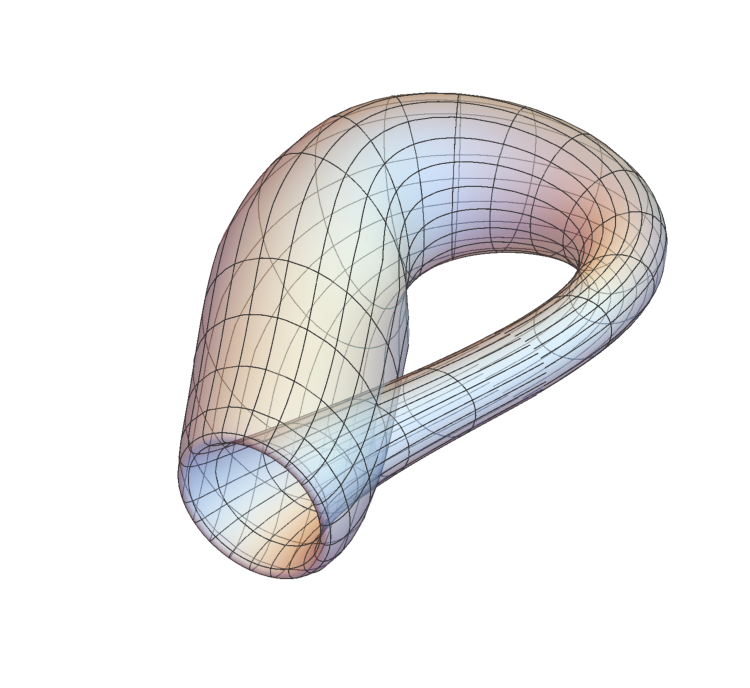
\includegraphics{./images/ch12/KleinBottle.pdf}}
	\end{center}	
\end{shaded}

[分析]:通过$\Sigma$上任一点处垂直于曲面的流速为$\bm{v}\cdot\bm{n}$
($\bm{n}$沿曲面正向的单位法向量),设$\d S$为$\Sigma$上的面积微元,
则流量微元为$\bm{v}\cdot\bm{n}\d S$。从而通过$\Sigma$的总流量
$$\Phi=\iint\limits_{\Sigma}\bm{v}\cdot\bm{n}\d S.$$
如果我们记$\d\bm{S}=\bm{n}\d S$,则上式亦可表示为
$$\Phi=\iint\limits_{\Sigma}\bm{v}\cdot\d\bm{S}.$$

与对坐标的曲线积分类似,注意到
$$\bm{n}\d S=(\pm\d\sigma_{yz},\pm\d\sigma_{zx},\pm\d\sigma_{xy})
=(\pm\d y\d z,\pm\d z\d x,\pm\d x\d y),$$
故通常将前式记为\ps{为了符号简洁,暂时忽略面积微元前面的符号,待实际计算时再具体讨论}
$${\Phi=\iint\limits_{\Sigma}P(x,y,z)\d y\d z
+Q(x,y,z)\d z\d x+R(x,y,z)\d x\d y}.$$
这种形式的积分称为{\it 对坐标(第二型)的曲面积分}。

\begin{thx}
	{\bf 第二型曲面积分的计算:}例如,已知曲面$\Sigma:\,z=f(x,y),\,(x,y)\in D$,计算
	$$I=\iint\limits_{\Sigma}R(x,y,z)\d x\d y$$	
	\begin{enumerate}[Step-1\;]
% 	  \setlength{\itemindent}{1cm}
	  \item 观察原积分,确定积分变量为$x$和$y$
	  \item 以$x,y$为自变量,给出曲面方程
	  $$z=z(x,y),\;(x,y)\in D$$ 
	  \item 写出对应的二重积分
	  $$\iint\limits_DR(x,y,z(x,y))\d\sigma_{xy}$$
	  \item {\b 根据曲面方向确定积分的符号}:{\it 若曲面正向与$z$轴正向成锐角,取正号;
	  反之为负},从而
	  $${I=\pm\iint\limits_DR(x,y,z(x,y))\d\sigma_{xy}}$$
	  \item 计算积分
	\end{enumerate}
\end{thx}

{\bf 注:}计算对坐标的曲线积分也可以采用与以上类似的步骤来描述。

例如,考虑对坐标的曲线积分
$$I=\int_Lf(x,y)\d x.$$
首先确定$x$为积分变量,然后以$x$为自变量给出曲线的方程
$$L:\;y=y(x),\;x\in[a,b].$$
接下来,写出对应的定积分(上限大于下限)
$$\int_a^bf(x,y(x))\d x,$$
再{\b 根据曲线的方向确定积分的符号}(
{\it 若曲线方向和$x$轴正向的夹角为锐角,取正号,反之为负}),从而
$$I=\pm\int_a^bf(x,y(x))\d x.$$
最后计算积分。

{\bf 例:}已知$\Sigma$为$x+y+z=1$与各坐标面所围立体的外表面,计算
$$\oiint\limits_{\Sigma}x^2\d x\d y$$

{\bf 例:}计算曲面积分
$$I=\oiint\limits_{\Sigma}xyz\d x\d y,$$
其中$\Sigma$由四分之一单位球面($x\geq 0,y\geq 0$)和
$x=0,y=0$共同组成。

% \subsection{曲面积分的应用}
% 
% \begin{enumerate}
%   \setlength{\itemindent}{1cm}
%   \item {\bf 对面积的曲面积分:} 
%   \begin{itemize}
%     \item 曲面的质量 
%     \item 质心 
%     \item 转动惯量 
%     \item 万有引力 
%   \end{itemize}
%   \item {\bf 对坐标的曲面积分:} 
%   \begin{itemize}
%     \item 流量
%   \end{itemize}
% \end{enumerate}

{\bf 例:}已知流速场$\bm{v}=(0,yz,z^2)$,求穿过柱面
$y^2+z^2=1(z\geq 0)$被$x=0$和$x=1$所夹部分的流量,
取曲面上侧为其正向。

{\bf 例:}将半径为$R$的球体置于水中,顶部与水面相切,求球的上半部分所受水的压力。

\begin{ext}
	{\bf 课后作业}
	\begin{enumerate}
	  \item 已知$\Sigma$是由上半单位球面与$xOy$坐标面所围的立体的外表面,
	  计算$\ds\iint_{\Sigma}(x^2+y^2+z^2)\d x\d y$。
	  \item 已知$\S$为椭球面$\df{x^2}{a^2}+\df{y^2}{b^2}+\df{z^2}{c^2}=1$
	  的上半部分的上侧,计算$\ds\iint_Sx^3\d y\d z+y^2\d z\d x$。
	  \item 求向量场$(y,x,z)$通过柱面$S:x^2+y^2=1,0\leq z\leq 1$的流量,
	  其中取$S$的外侧为其正向。
	  \item 设$\Sigma$为平面$x+y+z=1$在第一卦限的上侧,$f(x,y,z)$连续,证明:
	  $\ds\iint_{\Sigma}[f(x,y,z)+x]\d y\d z-[2f(x,y,z)-y]\d z\d x+
	  [f(x,y,z)+z]\d x\d y=\df12$。(提示:化为第一型的曲面积分计算)
	\end{enumerate}
\end{ext}

\section{Gauss公式和Stokes公式}

{\bf Green公式:}
$$\oint_LP(x,y)\d x+Q(x,y)\d y=\iint\limits_D\left(
\df{\p Q}{\p x}-\df{\p P}{\p y}\right)\d\sigma $$
其中:
\begin{itemize}
  \item {$D$:}$xOy$平面内的{\it 有界闭区域}
  \item {$L=\p D$:}分段光滑曲线,按{\it “左侧法则”}取正向
  \item {$P(x,y),Q(x,y)$:}在$D$内有连续偏导数
\end{itemize}

\subsection{Green公式流量形式的三维推广——Gauss公式}

{\bf Green公式:}平面向量场$\bm{v}$,平面区域$D$,$L=\p D$
$${\oint_L\bm{v}\cdot\bm{n}\d s=\iint\limits_D\mathrm{div}\,\bm{v}\d\sigma}$$

{\bf 推广:}空间向量场$\bm{v}$, 空间区域$\Omega$, $\Sigma=\p\Omega$
$${\oiint\limits_{\Sigma}\bm{v}\cdot\bm{n}\d
S=\iiint\limits_{\Omega}\mathrm{div}\,\bm{v}\d V}$$

\begin{thx}
	{\bf Gauss公式}
	$$\oiint\limits_{\Sigma}P\d y\d z+Q\d z\d x+R\d x\d y=\iiint\limits_{\Omega}
	\left(\df{\p P}{\p x}+\df{\p Q}{\p y}+\df{\p R}{\p z}\right)\d V$$
	其中:
	\begin{itemize}
% 	  \setlength{\itemindent}{1cm}
	  \item {$\Omega$:}空间{\it 有界闭区域}
	  \item {$\Sigma=\p\Omega$:}分片光滑曲面,取{\it “外侧”}为正向
	  \item {$P(x,y,z),Q(x,y,z),R(x,y,z)$:}在$\Omega$内偏导连续
	\end{itemize}
\end{thx}

{\bf 教材-例1:}设向量场$\bm{v}=(x,y,z)$,$\Sigma:x^2+y^2+z^2=R^2$,试验证
Gauss公式。

{\bf 教材-例2:}求流速场$\bm{v}=(x,y,z)$由内向外流过$\Sigma:x^2+y^2=R^2
(0\leq z\leq H)$侧面的流量。

{\bf 教材-例3:}设原点处有一电量为$e$的点电荷,求其产生的静电场通过曲面
$$\df{x^2}{a^2}+\df{y^2}{b^2}+\df{z^2}{c^2}=1$$
的电通量。

[提示]:{\it 电场强度:}${E=\df{ke}{r^2}}$

{\bf 例:}设$\Sigma$为曲面$z=\sqrt{x^2+y^2}$及平面$z=1$和$z=2$
所围立体的外表面,求
$$\oiint\limits_{\Sigma}\sqrt{x^2+y^2}e^z(\d y\d z+\d z\d x+\d x\d y)$$

[提示]:使用Gauss公式,结果为$\df43\pi e(e+1)$.

{\bf 例:}设$\Sigma$为锥面$z=\sqrt{x^2+y^2}(0\leq z\leq 1)$的下侧,则
$\ds\iint_{\Sigma}x\d y\d z+2y\d z\d x+3(z-1)\d x\d y=2\pi$

[提示]:“补全”曲面,用Gauss公式计算!

\begin{shaded}
	{\bf Gauss公式 vs. NUDT}
	
	Gauss公式是各种考试的常客,在NUDT也不例外:P,尤其是各种需要“补全”的问题:
	
	{\bf NUDT-2016春}:计算曲面积分
	$$\oiint\limits_{\Sigma}2(1+x)\d y\d z+yz\d x\d y,$$
	其中$\Sigma$是曲线$y=\sqrt x\;(0\leq x\leq 1)$绕$x$轴旋转
	一周所得的曲面,且法方向与$x$轴正向的夹角大于$\pi/2$.
	
	[提示]:先进行“补全”,然后利用Gauss公式计算补全后的积分,再删除补全的部分,
	结果为$-3\pi$.
	
	{\bf NUDT-2015春}:设曲面$S$为锥面$z=\sqrt{x^2+y^2}\;(0\leq z\leq2)$,
	法向量指向上侧,求流速场$\bm{v}=xz\bm{i}-yz\bm{j}+z^2\bm{k}$通过
	曲面$S$的流量。
	
	[提示]:补全后,使用Gauss公式,结果:$8\pi$。
	
	{\bf NUDT-2014春}:已知$\Sigma$为柱面$x^2=y^2=1\;(0\leq z\leq1)$
	的外侧,计算曲面积分
	$$I=\iint\limits_{\Sigma}(x+y\sin z)\d y\d z+(z+xe^y)\d x\d y$$
	
	[提示]:补全后,使用Gauss公式,结果:$\pi$。
	
	{\bf NUDT-2013春}:已知流体的流动速度为$\bm{v}=(x^2+y+1,y^2+z+1,
	z^2+x+1)$,求其通过曲面$\Sigma:\;z=\sqrt{1-x^2-y^2}$上侧的流量。
	
	[提示]:补全后,使用Gauss公式,结果:$\df32\pi$。
	
	{\bf NUDT-2012春}:设$S$为锥面$x^2+y^2=z^2$对应于$0\leq z\leq 1$
	的部分的外侧,计算积分
	$$I=\iint\limits_S(x^3-z)\d y\d z+(y^3-x)\d z\d x
	+(x-y^2)\d x\d y$$
	
	[提示]:补全后,使用Gauss公式,结果:$\df{11}{20}\pi$。
	
	{\bf NUDT-2011春}:已知$\Sigma$为曲线$y^2=2z\;(0\leq z\leq 4)$
	绕$z$轴旋转一周而成的曲面,其法向量与$z$轴正向成锐角,计算积分
	$$\iint\limits_{\Sigma}xz\d y\d z+x^2y\d z\d x+y^2z\d x\d y$$
	
	[提示]:补全后,使用Gauss公式,结果:$-\df{64}{3}\pi$。
	
	{\bf NUDT-2011春}:求流速为$\bm{v}=xz\bm{i}+yx\bm{j}+zy\bm{k}$
	的流体流过曲面$S$下侧的流量,其中$S$为$z=\sqrt{x^2+y^2}$介于$z=1$和
	$z=2$之间的部分。
	
	[提示]:补全后,使用Gauss公式,结果:$\df{15}{4}\pi$。
	
	注意,正确区分积分的类型是解题的第一步!有些时候Gauss公式并不是最好的选择。
	
	{\bf NUDT-2015春}:
	设$\Sigma$为上半球面$x^2+y^2+z^2=4x\;(z\geq 0)$
	夹在圆柱$x^2+y^2=2x$内的部分,$\bm{n}=(\cos\alpha,\cos\beta,\cos\gamma)$
	为该半球面在点$(x,y,z)$处指向上侧的单位法向量,计算积分
	$$I=\iint\limits_{\Sigma}[(y-z)\cos\alpha+(z-x)\cos\beta
	+(x-y)\cos\gamma]\d S$$
	
	[提示]:本题若使用Gauss公式,计算并不能得到很好地简化,因此,直接计算第一型曲面积分即可。
	事实上,$\bm{n}=\df12\left(x-2,y,z\right).$
	带入化简后,再利用对称性,可得
	$$I=\iint\limits_{\Sigma}(z-y)\d S=\iint\limits_{\Sigma}z\d S$$
	
	又$z=\sqrt{4x-x^2-y^2},(x,y)\in D$,其中$D:x^2+y^2\leq2x$,
	$\d S=\df2z\d\sigma_{xy}$,故
	$$I=\iint\limits_{\Sigma}z\d S=2\iint\limits_{D}z\d S=2\pi$$
\end{shaded}

{\bf 例}(同济11-6-例2):计算曲面积分
$$\iint\limits_{\Sigma}(x^2\cos\alpha+y^2\cos\beta
+z^2\cos\gamma)\d S,$$
其中$\Sigma$为$x^2+y^2=z^2$介于$z=0$和$z=h\;(h>0)$之间的部分的下侧,
$\cos\alpha,\cos\beta,\cos\gamma$为$\Sigma$在点$(x,y,z)$处的法向量
的方向余弦。

[提示]:补全,Gauss公式,结果$-\df12\pi h^4$.

\begin{shaded}
	{\bf Green第一公式:}设$u(x,y,z)$和$v(x,y,z)$在空间闭区域$\Omega$上
	具有二阶连续偏导数,则
	$$
	\oiint\limits_{\Sigma}u\bigtriangledown v\cdot\bm{n}\d S
	=\iiint\limits_{\Omega}(u\Delta v
	+\bigtriangledown u\cdot\bigtriangledown v)\d V
	$$ 
	其中:$\Sigma=\p\Omega$取外侧为正,$\bm{n}$为$\Sigma$的单位法向量,Laplace
	算子$\Delta=\df{\p^2}{\p x^2}+\df{\p^2}{\p y^2}+\df{\p^2}{\p z^2}$.
		
	{\bf Green第二公式:}与以上公式条件相同,则有
	$$
	\oiint\limits_{\Sigma}\left(u\bigtriangledown v
	-v\bigtriangledown u\right)\cdot\bm{n}\d S=
	\iiint\limits_{\Omega}(u\Delta v-v\Delta u)\d V
	$$
\end{shaded}



{\bf 散度与无源场}

{\it 散度(流量密度、通量密度):}
$$\mathrm{div}\,\bm{v}=\df{\p P}{\p x}+\df{\p Q}{\p y}+\df{\p R}{\p
z}=\bigtriangledown\cdot\bm{v}$$ 

{\it 无源场:}
$${\mathrm{div}\,\bm{v}=0}$$ 

{\bf 定理2}若向量场$\bm{v}$在空间区域$\Omega$内为无源场,则
其通过$\Omega$边界的流量为$0$。

{\bf 散度的运算法则}

已知$\bm{v}=(P,Q,R)$,$u=u(x,y,z)$,$C\in\mathbb{R}$, 
其中$P,Q,R,u$均可微,则\ps{请牢记!}
\begin{enumerate}[(1)]
  \setlength{\itemindent}{1cm}
  \item ${\mathrm{div}(C\bm{v}) =C\,\mathrm{div}\,\bm{v}}$ 
  \item ${\mathrm{div}(u\bm{v}) =u\,\mathrm{div}\,\bm{v}
  +\bm{v}\cdot\bigtriangledown u}$
\end{enumerate}

\begin{shaded}
	{\bf Gauss公式的“挖洞”问题}
	
	和Green公式类似,Gauss公式也有需要“挖洞”处理的问题。具体的处理方法
	参见Green公式的“挖洞”处理。
	
	{\bf 教材-例4:}(Gauss积分)计算
	$$I(\xi,\eta,\zeta)=\oiint\limits_{\Sigma}
	\df{\cos(\bm{r},\bm{n})}{|\bm{r}|^2}\d S,$$
	其中:$\Sigma$为不经过点$P(\xi,\eta,\zeta)$的光滑闭曲面,
	$\bm{n}$为$\Sigma$上任一点$M$处指向外侧的单位法向量,
	$\bm{r}=\bm{MP}$。
	
	几何意义:曲面在以$P$为球心的单位球上的投影面积(内侧为正)。
	
	{\bf 例:}设$\Sigma$为$2x^2+2y^2+z^2=4$的外侧,求
	$$\oiint\limits_{\Sigma}\df{x\d y\d z+y\d z\d x+z\d x\d
	y}{(x^2+y^2+z^2)^{3/2}}$$
	
	[提示]:可以验证,在原点之外旋度为零,“挖洞”后使用Gauss公式!
	
	{\bf 思考:}上例中的积分改成
	$$\oiint\limits_{\Sigma}\df{x\d y\d z+y\d z\d x+z\d x\d y}
	{(x^2+2y^2+2z^2)^{3/2}}$$
	该如何计算?
	
	[提示]:挖一个椭球形状的“洞”:$x^2+2y^2+2z^2=\e$
\end{shaded}



% {\it 二维形式的Gauss积分:}
% $$I=\int_L\df{\cos(\bm{r},\bm{n})}{|\bm{r}|}\d s,$$
% 
% 几何意义:曲线在以$P$为圆心的单位圆上的投影弧长(顺时针方向为正)。

\subsection{Green公式环量形式的三维推广——Stokes公式}

{\bf Green公式:}平面向量场$\bm{v}$,平面区域$D$,$L=\p D$ 
$${\oint_L\bm{v}\cdot\bm{T}\d s=\iint\limits_D
\left(\df{\p Q}{\p x}-\df{\p P}{\p y}\right)\d\sigma}$$
 
{\it 三维推广:} 空间向量场$\bm{v}$, 空间曲线$L$, $L=\p\Sigma$ 
\begin{eqnarray*}
	{\ds\oint_L\bm{v}\cdot\bm{T}\d s}&{=}&
	{\ds\iint\limits_{\Sigma^+}\left(\df{\p R}{\p y}-\df{\p Q}{\p
	z}\right)\d\sigma_{yz}}\\ 
	&& {\hspace{-3cm}\ds\iint\limits_{\Sigma^+}\left(\df{\p P}{\p
	z}-\df{\p R}{\p x}\right)\d\sigma_{zx}
	+\iint\limits_{\Sigma^+}\left(\df{\p Q}{\p x}-\df{\p P}{\p
	y}\right)\d\sigma_{xy}}
\end{eqnarray*}

{\bf 定理:}(Stokes公式)
\begin{eqnarray*}
	{\ds\oint_L\bm{v}\cdot\bm{T}\d s}&{=}&
	{\ds\iint\limits_{\Sigma^+}\left(\df{\p R}{\p y}-\df{\p Q}{\p
	z}\right)\d\sigma_{yz}}\\ 
	&& {\hspace{-2cm}\ds\iint\limits_{\Sigma^+}\left(\df{\p P}{\p
	z}-\df{\p R}{\p x}\right)\d\sigma_{zx}
	+\iint\limits_{\Sigma^+}\left(\df{\p Q}{\p x}-\df{\p P}{\p
	y}\right)\d\sigma_{xy}}
\end{eqnarray*}
其中
\begin{itemize}
  \item {$\Sigma$:}空间光滑曲面
  \item {$L=\p\Sigma$:}空间光滑闭曲线,按{“右手法则”}取正向
  \item {$P,Q,R$:}在包含$\Sigma$的空间区域内偏导连续
\end{itemize}

{\bf 例:}设向量场$\bm{v}=(-z,y,x)$,曲线$L$为$x^2+z^2=1$与$y=2$的交线,
由$y$轴正向看过去为逆时针方向,$\Sigma$为以$L$为边界的圆盘,正向与$y$
轴正向一致,试验证Stokes公式。

{\bf 例:}计算积分
$$I=\oint_Lx^2y\d x+y^2\d y+z\d z,$$
其中$L$为$x^2+y^2=1$与$x+z=1$的交线,从$z$轴正向看过去为
逆时针方向。

{\it 旋度:}
$${\mathrm{rot}\,\bm{v}=\left(
\df{\p R}{\p y}-\df{\p Q}{\p z},
\df{\p P}{\p z}-\df{\p R}{\p x},
\df{\p Q}{\p x}-\df{\p P}{\p y}
\right)}$$ 
{记号:}
$$\mathrm{rot}\,\bm{v}\quad \mbox{或}\quad\mathrm{curl}\,\bm{v}$$ 

{\bf Stokes公式的向量形式:}
$${\oint_L\bm{v}\cdot\bm{T}\d s
=\iint\limits_{\Sigma}\mathrm{rot}\,\bm{v}\cdot\bm{n}\d S}$$

{\bf 旋度的行列式表示}

$${\mathrm{rot}\,\bm{v}=\bigtriangledown\times\bm{v} 
=\left|\begin{array}{ccc}
	\bm{i} & \bm{j} & \bm{k}\\
	\df{\p}{\p x} & \df{\p}{\p y} & \df{\p}{\p z}\\
	P & Q & R
\end{array}\right|}$$ 

{\bf Stokes公式的行列式形式:} 
$${\oint_LP\d x+Q\d y+R\d z=\iint\limits_{\Sigma}
\left|\begin{array}{ccc}
	\d y\d z & \d z\d x & \d x\d y\\
	\df{\p}{\p x} & \df{\p}{\p y} & \df{\p}{\p z}\\
	P & Q & R
\end{array}\right|}$$

{\bf 旋度的运算法则}

{\bf 已知:}$\bm{v}=(P,Q,R)$,$u=u(x,y,z)$,$C\in\mathbb{R}$, 
其中$P,Q,R,u$均可微, 则
\begin{enumerate}[(1)]
  \setlength{\itemindent}{1cm}
  \item ${\mathrm{rot}(C\bm{v}) =C\,\mathrm{rot}\,\bm{v}}$ 
  \item ${\mathrm{rot}(u\bm{v}) =u\,\mathrm{rot}\,\bm{v}
  +\bigtriangledown u\times\bm{v}}$
\end{enumerate}

{\it 无旋场:}
$${\mathrm{rot}\,\bm{v}=0}$$ 

{\bf 定理4:}
对空间向量场$\bm{v}$,以下条件等价: 
\begin{enumerate}[(1)]
  \setlength{\itemindent}{1cm}
  \item $\bm{v}$为无旋场; 
  \item $\bm{v}$为保守场(积分与路径无关); 
  \item $\bm{v}$存在势函数。
\end{enumerate}

{\bf 例:}验证$\bm{F}=\left(x^2,yz,\df{y^2}2\right)$为保守场,并求其势函数。

{\bf 例:}刚体绕经过坐标原点的某一轴$l$以角速度$\bm{\omega}$旋转,求其上任一点处
线速度$\bm{v}$的旋度。

$${\bm{v}=\bm{\omega}\times\bm{r}}$$

{\it 旋度:}曲面上某一点处,垂直于曲面法向量的旋转强度

{\bf 例:}利用Stokes公式计算积分
$$\oint_Lz\d x+x\d y+y\d z,$$
其中$L$为$x+y+z=1$被三个坐标面所截成的三角形的边界,其正向
与该三角形上侧的法向量满足右手法则。

{\bf 例:}利用Stokes公式计算积分
$$\oint_L(y^2-z^2)\d x+(z^2-x^2)\d y+(x^2-y^2)\d z,$$
其中$L$为平面$x+y+z=\df 32$截立方体$0\leq x,y,z\leq 1$
的截痕,从$x$轴正向看去,取逆时针方向。

{\bf 思考:}找出以下推导中存在的问题
$\Omega:r\leq R$,$\Sigma=\p\Omega$,取外侧,
$r=\sqrt{x^2+y^2+z^2}$

(1)
\begin{align*}
	\ds\oiint\limits_{\Sigma}&\df{x^3}{r^3}\d
  	y\d z+\df{y^3}{r^3}\d z\d x+\df{z^3}{r^3}\d x\d y
  	=\df 1{R^3}\oiint\limits_{\Sigma}x^3\d y\d z+y^3\d z\d x+z^3\d
  	x\d y\\
  	&=\df 1{R^3}\iiint\limits_{\Omega}3r^2\d V{=\df
  3R\iiint\limits_{\Omega}\d V} =4\pi R^2
\end{align*}

(2)
$$\ds\oiint\limits_{\Sigma}\df{x^3}{r^3}\d
  	y\d z+\df{y^3}{r^3}\d z\d x+\df{z^3}{r^3}\d x\d y
  	=\ds\iiint\limits_{\Omega}\left[\df{\p}{\p x}\df{x^3}{r^3}+\df{\p}{\p
  	y}\df{y^3}{r^3}+\df{\p}{\p z}\df{z^3}{r^3}\right]\d V$$

{\bf 例:}设$r=\sqrt{x^2+y^2+z^2}$,则\ps{这个结果最好能够作为公式记住!}
\begin{enumerate}[(1)]
  \setlength{\itemindent}{1cm}
  \item $\mathrm{div}(\bigtriangledown\,r)=\df 2r$
  \item $\mathrm{rot}(\bigtriangledown\,r)=0$
\end{enumerate}

\begin{shaded}
	{\bf 关于原函数的计算}	
	
	{\bf 习题12.2-8}(2)计算如下微分形式的原函数
	$$yz(2x+y+z)\d x+xz(x+2y+z)\d y+xy(x+y+2z)\d z.$$
	
	[方法一]:({\it 折线法})考虑积分路径$(0,0,0)\to(x,0,0)\to(x,y,0)\to(x,y,z)$
	(注:类似的路径应该共有6条!)
	,则
	\begin{align*}
		u(x,y,z)&=\int_{(0,0,0)}^{(x,y,z)}P\d x+Q\d y+R\d z+C\\
		&=\dint_{(0,0,0)}^{(x,0,0)}yz(2x+y+z)\d x
		+\dint_{(x,0,0)}^{(x,y,0)}xz(x+2y+z)\d y\\
		&\quad+\dint_{(x,y,0)}^{(x,y,z)}xy(x+y+2z)\d z+C\\
		&=0+0+\dint_{(x,y,0)}^{(x,y,z)}xy(x+y+2z)\d z+C\\
		&=x^2yz+xy^2z+xyz^2+C
	\end{align*}
	
	[方法二]:({\it “凑”微分})(注:以下用到了微分公式:$\d(uvw)=uv\d w+uw\d v+vw\d u$)
	\begin{align*}
		yz&(2x+y+z)\d x+xz(x+2y+z)\d y+xy(x+y+2z)\d z\\
		&=yz\d x^2+y^2z\d x+yz^2\d x\\
		&+x^2z\d y+xz\d y^2+xz^2\d y\\
		&+x^2y\d z+xy^2\d z+xy\d z^2\\
		&=\d(x^2yz+xy^2z+xyz^2)
	\end{align*}
	故$u=xyz(x+y+z)+C$
	
	[方法三]:({\it 逐项积分})由本题条件$u'_x=yz(2x+y+z)$,两边关于$x$积分(视
	$y,z$为常数),可得$u=x^2yz+xyz(y+z)+v(y,z)$,其中$v(y,z)$待定。进而
	$$u'_y=x^2z+2xyz+xz^2+v'_y.$$	
	
	又由题意,$u'_y=xz(x+2y+z)$,故$v'_y=0$,
	两边关于$y$积分(视$z$为常数),从而$v=w(z)$,其中$w(z)$待定。进而
	$$u'_z=x^2y+xy^2+2xyz+v'_z=x^2y+xy^2+2xyz+w'_z.$$
	
	再由$u'_z=xy(x+y+2z)$,故$w'_z=0$,从而$w=C\;(C\in\mathbb{R})$。
	
	综上,
	$$u=x^2yz+xyz(y+z)+v(y,z)=x^2yz+xyz(y+z)+w(z)=x^2yz+xyz(y+z)+C.$$
	
\end{shaded}

\newpage

\section{对称性在积分计算中的应用}

\bigskip

{\bf 1、定积分中的对称性}

{\bf (1)对称区间上的积分}

{\it\b 奇函数在对称区间上的积分}:
若$f(x)$为奇函数,则\ps{利用变量替换即可证明}
$$\int_{-a}^0f(x)\d x=-\int_0^af(x)\d x,$$
从而
$${\b \int_{-a}^af(x)\d x=0}.$$

{\it\b 偶函数在对称区间上的积分}:若$f(x)$为偶函数,则
$$\int_{-a}^0f(x)\d x=\int_0^af(x)\d x,$$
从而
$${\b \int_{-a}^af(x)\d x=2\int_0^af(x)\d x}.$$

例如:$\dint_{-1}^{1}\df{|x|+\sin x}{1+x^2}\d x
=2\dint_0^{1}\df{x}{1+x^2}\d x=\ldots$

{\bf (2)图像对称性的函数的积分}

{\it 图像关于$x=a$对称的函数}:已知$f(x)=g(2a-x)$
\ps{这说明$y=f(x)$和$y=g(x)$的图像关于$x=a$对称},则
$$\int_{a-b}^{a+b}f(x)\d x=\int_{a-b}^{a+b}g(x)\d x.$$

推论:{\b $\dint_0^{\frac{\pi}2}f(\sin x)\d x=\dint_0^{\frac{\pi}2}f(\cos x)\d x$}

例如:$\dint_0^{\frac{\pi}2}\df{\cos^3x\d x}{\cos^3x+\sin^3x}
=\dint_0^{\frac{\pi}2}\df{\sin^3x\d x}{\sin^3x+\cos^3x}
=\df12\dint_0^{\frac{\pi}2}\df{\sin^3x+\cos^3x}{\cos^3x+\sin^3x}\d x=\df{\pi}4$

{\it\b 函数图像的对称翻转}:\ps{注意到$y=f(x)$和$y=f(2a-x)$的图像关于$x=a$对称}
$$\int_{a-b}^{a+b}f(x)\d x=\int_{a-b}^{a+b}f(2a-x)\d x.$$
更为常用的形式是
$${\b \int_0^af(x)\d x=\int_0^af(a-x)\d x}.$$

例如:$\dint_0^1\df{e^x\d x}{e^{1-x}+e^x}
=\dint_0^1\df{e^{1-x}\d x}{e^x+e^{1-x}}
=\df12\dint_0^1\df{e^x+e^{1-x}}{e^x+e^{1-x}}\d x=\df12$

\bigskip

{\bf 2、二重积分中的对称性}\ps{重点掌握,深入理解,再推广应用到其他的积分上}

以下考虑二重积分
$$\ds\iint\limits_Df(x,y)\d\sigma.$$

{\bf(1)关于某个坐标轴对称的区域上的积分}

设积分区域$D$关于$x=0$对称\ps{关于$y=0$对称的相关结论是类似的。\b 验证$D$关于$x=0$对称,只需
在$D$的表示中用$-x$代换$x$,若所得区域不变,即证},
$D_1,D_2$分别为$D$中对应于$x\geq0$和$x\leq0$的部分。

{\it\b 被积函数关于$x$为奇函数}:若$f(-x,y)=-f(x,y)$,则
$$\ds\iint\limits_{D_1}f(x,y)\d\sigma=-\ds\iint\limits_{D_2}f(x,y)\d\sigma,$$
从而
$${\b \ds\iint\limits_{D}f(x,y)\d\sigma=0}$$

{\it\b 被积函数关于$x$为偶函数}:若$f(-x,y)=f(x,y)$,则
$$\ds\iint\limits_{D_1}f(x,y)\d\sigma=\ds\iint\limits_{D_2}f(x,y)\d\sigma,$$
从而
$${\b\ds\iint\limits_{D}f(x,y)\d\sigma=2\ds\iint\limits_{D_2}f(x,y)\d\sigma}.$$

例如:$\ds\iint\limits_{|x|+|y|\leq1}\df{x^2}{x^2+y^2}\d\sigma
=4\ds\iint\limits_{|x|+|y|\leq1\atop{x\geq0,y\geq0}}\df{x^2}{x^2+y^2}
\d\sigma$

{\bf(2)关于$y=x$对称的区域上的积分}

设积分区域$D$关于$y=x$对称\ps{这意味着在$D$的表示中交换$x$和$y$,所得区域仍为$D$,例如:
$x^2+y^2\leq 1$,有时我们也称之为$x,y$在$D$内可交换或地位相同},
$D_1,D_2$分别为$D$中对应于$y\geq x$和$y\leq x$的部分。

{\it\b 轮换对称}:
$$\ds\iint\limits_{D_1}f(x,y)\d\sigma=\ds\iint\limits_{D_2}f(y,x)\d\sigma,$$
从而可知
$${\b\ds\iint\limits_{D}f(x,y)\d\sigma=\ds\iint\limits_{D}f(y,x)\d\sigma}.$$
这个性质可以描述为:{\it 若在$D$的表示中,$x,y$是可交换的,则在$D$上的积分中$x,y$也是可交换的}。

例如:$\ds\iint\limits_{|x|+|y|\leq1\atop{x\geq0,y\geq0}}\df{x^2}{x^2+y^2}\d\sigma
=\ds\iint\limits_{|x|+|y|\leq1\atop{x\geq0,y\geq0}}\df{y^2}{y^2+x^2}\d\sigma
=\df12\ds\iint\limits_{|x|+|y|\leq1\atop{x\geq0,y\geq0}}\df{x^2+y^2}{x^2+y^2}\d\sigma
=\df{\pi}8
$

{\it\b 变量可交换}:若{\b$f(x,y)=f(y,x)$}
\ps{这意味着在$f(x,y)$中交换变量$x,y$的位置,函数值不变},则
$$\ds\iint\limits_{D_1}f(x,y)\d\sigma=\ds\iint\limits_{D_2}f(x,y)\d\sigma,$$
从而
$${\b\ds\iint\limits_Df(x,y)\d\sigma=2\ds\iint\limits_{D_1}f(x,y)\d\sigma}.$$

{\it\b 变量反对称}:若{\b $f(x,y)=-f(y,x)$},
\ps{这意味着在$f(x,y)$中交换变量$x,y$的位置,函数值反号}则
$$\ds\iint\limits_{D_1}f(x,y)\d\sigma=-\ds\iint\limits_{D_2}f(x,y)\d\sigma,$$
从而
$${\b\ds\iint\limits_{D}f(x,y)\d\sigma=0}.$$

例如:$D:0\leq x\leq 1,0\leq y\leq 1$,则
$\ds\iint\limits_D(x+y)\mathrm{sgn}(x-y)\d\sigma=0$

{\bf 练习题:}综合应用以上的对称性,求解如下积分:

i.\;$\ds\iint\limits_{x^2+y^2\leq 1}\df{(x+2y)^2}{1+x^2+y^2}\d\sigma$

ii.\;$\ds\iint\limits_{x^2+y^2\leq 1}\df{2x^2+x-y+1}{\sqrt{1-x^2-y^2}}\d\sigma$

iii.\;$\ds\iint\limits_D\df{a\sqrt{f(x)}+b\sqrt{f(y)}}{\sqrt{f(x)}+\sqrt{f(y)}}\d\sigma$,
其中$f(x)$恒为正,

\bigskip

{\bf 3、三重积分中的对称性}\ps{注意和二重积分比较}

{\bf(1)关于某个坐标面对称的区域上的积分}

{\it\b 被积函数关于某个变量为奇(偶)函数}:
空间区域$\Omega$关于$z=0$对称,$\Omega_1$为其中$z\geq 0$的部分,则
$${\b\iiint\limits_{\Omega}f(x,y,z)\d V=\left\{\begin{array}{ll}
0,& f(x,y,z)\mbox{关于}z\mbox{是奇函数}\\
2\ds\iiint\limits_{\Omega_1}f(x,y,z)\d V,& f(x,y,z)\mbox{关于}z\mbox{是偶函数}
\end{array}\right.}.$$

{\bf (2)轮换对称}

{\it\b 两个变量轮换}:区域{\b$\Omega$关于平面$y=x$对称}\ps{也即在$\Omega$的表示中,
$x,y$可以相互交换},则

$${\b\ds\iiint\limits_{\Omega}f(x,y,z)\d V=\iiint\limits_{\Omega}f(y,x,z)\d V}$$

例如:$\ds\iiint\limits_{x^2+y^2+z^2\leq R^2}\df{x^2-y^2}{(1+x^2+y^2+z^2)
^{3/2}}\d V
=\ds\iiint\limits_{x^2+y^2+z^2\leq R^2}\df{y^2-x^2}{(1+y^2+x^2+z^2)
^{3/2}}\d V=0
$

{\it\b 三个变量任意轮换:若区域$\Omega$中$x,y,z$地位相同
\ps{也即在$\Omega$的表示中$x,y,z$进行任意交换,所得区域不变。
例如:$\Omega:\;x^2+y^2+z^2\leq 1$},则积分
$\ds\iiint\limits_{\Omega}f(x,y,z)\d V$
中$x,y,z$的位置可以任意交换。}

例如:计算积分
$$\iiint\limits_{\Omega}(x+y+z)^2\d V,$$
其中$\Omega:\;\df{x^2}{a^2}+\df{y^2}{b^2}+\df{z^2}{c^2}\leq 1$。

利用关于$\Omega$坐标平面的对称性和被积函数的奇偶性,可得
$$\iiint\limits_{\Omega}(x+y+z)^2\d V
=\iiint\limits_{\Omega}(x^2+y^2+z^2)\d V.$$

其中,通过计算可得
$$\iiint\limits_{\Omega}z^2\d V=\df4{15}abc^3$$
注意到在$\Omega$中$\df xa,\df yb,\df zc$是可交换的,因此由轮换对称性,可得

$$\iiint\limits_{\Omega}x^2\d V=\df4{15}a^3bc,
\quad
\iiint\limits_{\Omega}x^2\d V=\df4{15}ab^3c.$$
综上,所求积分为$\df4{15}abc(a^2+b^2+c^2)$.

\bigskip

{\bf 4、对弧长的曲线积分中的对称性}

{\bf (1)关于某个坐标轴(面)对称的曲线上的积分}

{\it\b 被积函数为关于某个变量的奇(偶)函数}:曲线$L$关于$x=0$对称,$L_1$为其中$x\geq 0$的部分,则
\ps{这里给出的是平面曲线的例子,空间曲线上的曲线积分也有类似的性质}
$${\b\int_{L}f(x,y)\d s=\left\{\begin{array}{ll}
0,& f(x,y)\mbox{关于}x\mbox{是奇函数}\\
2\ds\int_{L_1}f(x,y)\d s,& f(x,y)\mbox{关于}x\mbox{是偶函数}
\end{array}\right.}$$

例如:$\ds\oint_{|x|+|y|=1}\df{x}{x^2+y^2}\d s=0$

{\bf (2)轮换对称}

{\it\b 3个变量的轮换}:\ps{类似地,也有关于两个变量轮换的结论}
{\b\;若曲线$L$上$x,y,z$地位相同,则积分$\ds\oint_Lf(x,y,z)\d s$
中$x,y,z$的位置可任意交换。}

例如:设$L$为$x^2+y^2+z^2=1$和$x+y+z=0$的交线,则
$$\oint_Lx^2\d s=\oint_Ly^2\d s=\oint_Lz^2\d s=\df13\oint_L(x^2+y^2+z^2)\d s
=\df23\pi$$

\bigskip

{\bf 5、对面积的曲面积分中的对称性}

{\bf (1)关于某个坐标面对称的曲面上的积分}

{\it\b 被积函数为关于某个变量的奇(偶)函数}:\;曲面{\b$\Sigma$关于$x=0$对称},
$\Sigma_1$为其中$x\geq 0$的部分,则
$${\b \iint\limits_{\Sigma}f(x,y,z)\d S=\left\{\begin{array}{ll}
0,& f(x,y,z)\mbox{关于}x\mbox{是奇函数}\\
2\ds\iint\limits_{\Sigma_1}f(x,y,z)\d S,& f(x,y,z)\mbox{关于}x\mbox{是偶函数}
\end{array}\right.}$$

例如:$\Sigma$为$x^2+y^2=R^2$在$z=0$和$z=1$间的部分,则
$\ds\iint\limits_{\Sigma}\df y{x^2+y^2+z^2}\d S=0$

{\bf (2)轮换对称}

{\it\b 3个变量的轮换}:\ps{类似地,也有关于两个变量轮换的结论}
\;曲面{\b$\Sigma$上$x,y,z$地位相同,则
$\ds\iint\limits_{\Sigma}f(x,y,z)\d S$
中$x,y,z$的位置可以任意交换}。

例如:设$\Sigma:x^2+y^2+z^2=R^2$,则
$$\ds\oiint\limits_{\Sigma}x^2\d S
=\ds\oiint\limits_{\Sigma}y^2\d S
=\ds\oiint\limits_{\Sigma}z^2\d S
=\df13\ds\oiint\limits_{\Sigma}(x^2+y^2+z^2)\d S=\df43\pi R^4,$$
进而可得
$$\ds\oiint\limits_{\Sigma}(x^2+3y^2)\d S=\df{16}{3}\pi R^4.$$

例如:设$S$为第一卦限中的半径为$a(a>0)$的球面,则
$$\oiint\limits_S xyz(y^2z^2+z^2x^2+x^2y^2)\d S
=3\oiint\limits_S x^3y^3z\d S=\ldots=\df{a^9}{32}$$

\bigskip

{\color{red}\hrule

\bigskip

\bf 总得来看,前面各类积分的对称性都是相似的,但是接下来在对坐标的
曲线和曲面积分中,对称性的有关结论将可能完全不同,请特别留意。
建议在对坐标的曲线和曲面积分中尽可能谨慎地使用对称性。

\bigskip

\hrule}

\bigskip

{\bf 6、对坐标的曲线积分中的对称性}

{\bf (1)关于某个坐标轴对称的曲线上的积分}

以如下积分为例\ps{空间曲线上对坐标的曲线积分有类似的性质}
$$\int_Lf(x,y)\d x$$

{\it\b 被积函数关于$x$为奇(偶)函数}:
\ps{此时的对称性与前面几类积分类似}
设曲线{\b$L$关于$x=0$对称},$L_1$为其中对应于
$x\geq0$的部分,则

$${\b\int_{L}f(x,y)\d x=\left\{\begin{array}{ll}
0,& f(x,y)\mbox{关于}x\mbox{是奇函数}\\
2\ds\int_{L_1}f(x,y)\d x,& f(x,y)\mbox{关于}x\mbox{是偶函数}
\end{array}\right.}$$

例如:$L$为逆时针的上半单位圆,则
$$\dint_Lx\d x=0,\quad\quad\quad \dint_Lx^2\d x=2\dint_{L_1}x^2\d x$$

\begin{shaded}
	证明思路:
	
	\begin{center}
		\resizebox{!}{4cm}{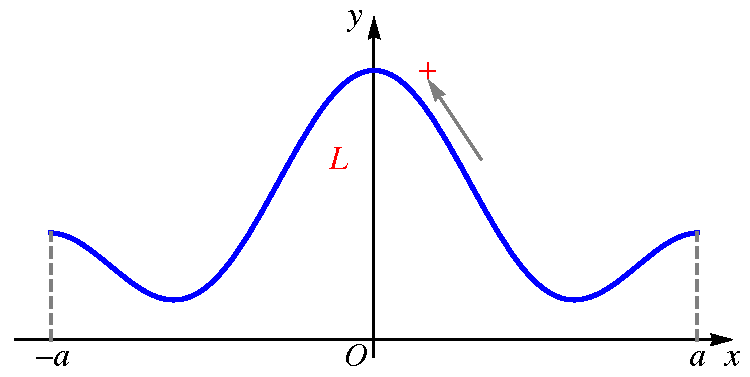
\includegraphics{./images/ch12/xdx.pdf}}
	\end{center}
	如图,$L$关于$x=0$对称(方向自右向左)。设$L$的方程为$y=y(x),(x\in[-a,a])$,则
	$y(-x)=y(x)$。记$L_1$和$L_2$分别为$L$上对应于$x\geq0$和$x\leq0$的部分。
	
	若$f(x,y)$关于$x$为奇函数(偶函数的情形证明类似),也即$f(-x,y)=-f(x,y)$,则	
	\begin{align*}
		\dint_{L_1}&f(x,y)\d x
		=\dint_{a}^{0}f(x,y(x))\d x
		=\dint_{a}^{0}f(x,y(-x))\d x
		=-\dint_{a}^{0}f(-x,y(-x))\d x\\
		&\xlongequal{u=-x}\dint_{-a}^{0}f(u,y(u))\d u
		=-\dint_{0}^{-a}f(u,y(u))\d u
		\dint_{L_2}f(x,y)\d x
	\end{align*}
	
	从而可知此时$\dint_{L}f(x,y)\d x=0$.
\end{shaded}

{\it\color{red} 被积函数关于$y$为奇(偶)函数}:\ps{\color{red} 之所以会有如下看起来
和前面结论完全相反的性质,是因为从$x$的方向看去,两部分积分曲线的方向正好是相反的!}
设曲线{\color{red} $L$关于$y=0$对称},$L_1$为其中对应于
$y\geq0$的部分,则

$${\color{red}\int_{L}f(x,y)\d x=\left\{\begin{array}{ll}
2\ds\int_{L_1}f(x,y)\d x,& f(x,y)\mbox{关于}y\mbox{是奇函数}\\
0,& f(x,y)\mbox{关于}y\mbox{是偶函数}
\end{array}\right.}$$

例如:设$L$为右半单位圆,取逆时针方向,则
$$\dint_Ly^2\d x=0,\quad\quad\quad \dint_Ly\d x=2\dint_{L_1}y\d x$$

\begin{shaded}
	证明思路:
	
	\begin{center}
		\resizebox{!}{6.5cm}{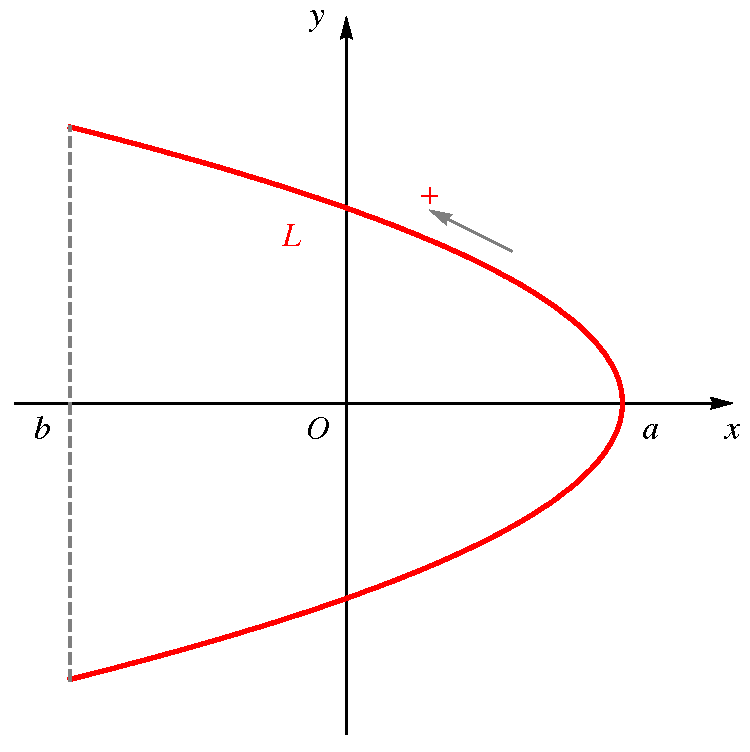
\includegraphics{./images/ch12/ydx.pdf}}
	\end{center}
	如图,$L$关于$y=0$对称(方向自下向上)。设$L$的方程为$y=\pm y(x),(x\in[a,b])$。
	记$L_1$和$L_2$分别为$L$上对应于$y\geq0$和$y\leq0$的部分。
	
	若$f(x,y)$关于$y$为奇函数(偶函数的情形证明类似),也即$f(x,-y)=-f(x,y)$,则
	\begin{align*}
		\dint_{L_1}&f(x,y)\d x
		=\dint_{a}^{b}f(x,y(x))\d x
		=-\dint_{a}^{b}f(x,-y(x))\d x\\
		&=\dint_{b}^{a}f(x,-y(x))\d x
		=\dint_{L_2}f(x,y)\d x
	\end{align*}
	
	从而可知此时$\dint_{L}f(x,y)\d x=2\dint_{L_1}f(x,y)\d x$.
\end{shaded}

{\bf (2)轮换对称}\ps{\color{red}平面曲线没有类似的性质!}

以空间曲线$L$上的积分
$$\int_Lf(x,y,z)\d x$$

{\it\color{red} $y,z$的轮换}:
\ps{类似地,若积分为$\int_Lf(x,y,z)\d y$,则在一定条件下可以考虑$y,z$的轮换}
{\color{red} 若$L$中$y,z$地位相同,则在积分$\int_Lf(x,y,z)\d x$
中$y,z$可交换位置},也即
$$\int_Lf(x,y,z)\d x=\int_Lf(x,z,y)\d x$$

{\color{red} 对于以上积分,任何时候都不可以考虑$x,y$或$x,z$的交换!}

\bigskip

{\bf 7、对坐标的曲面积分中的对称性}

以如下积分为例
$$\iint\limits_{\Sigma}f(x,y,z)\d x\d y$$

{\bf (1)关于某个坐标面对称的曲面上的积分}

{\it\b 被积函数关于$x$为奇(偶)函数}:\ps{关于$y$为奇(偶)函数的情形类似}
空间曲面{\b$\Sigma$关于$x=0$对称},$\Sigma_1$为其中$x\geq 0$的部分,则
$${\b\iint\limits_{\Sigma}f(x,y,z)\d x\d y=\left\{\begin{array}{ll}
0,& f(x,y,z)\mbox{关于}x\mbox{是奇函数}\\
2\ds\iint\limits_{\Sigma_1}f(x,y,z)\d x\d y,& f(x,y,z)\mbox{关于}x\mbox{是偶函数}
\end{array}\right.}$$

% [证明思路]:如图
% 
% \begin{center}
% 	\resizebox{!}{5cm}{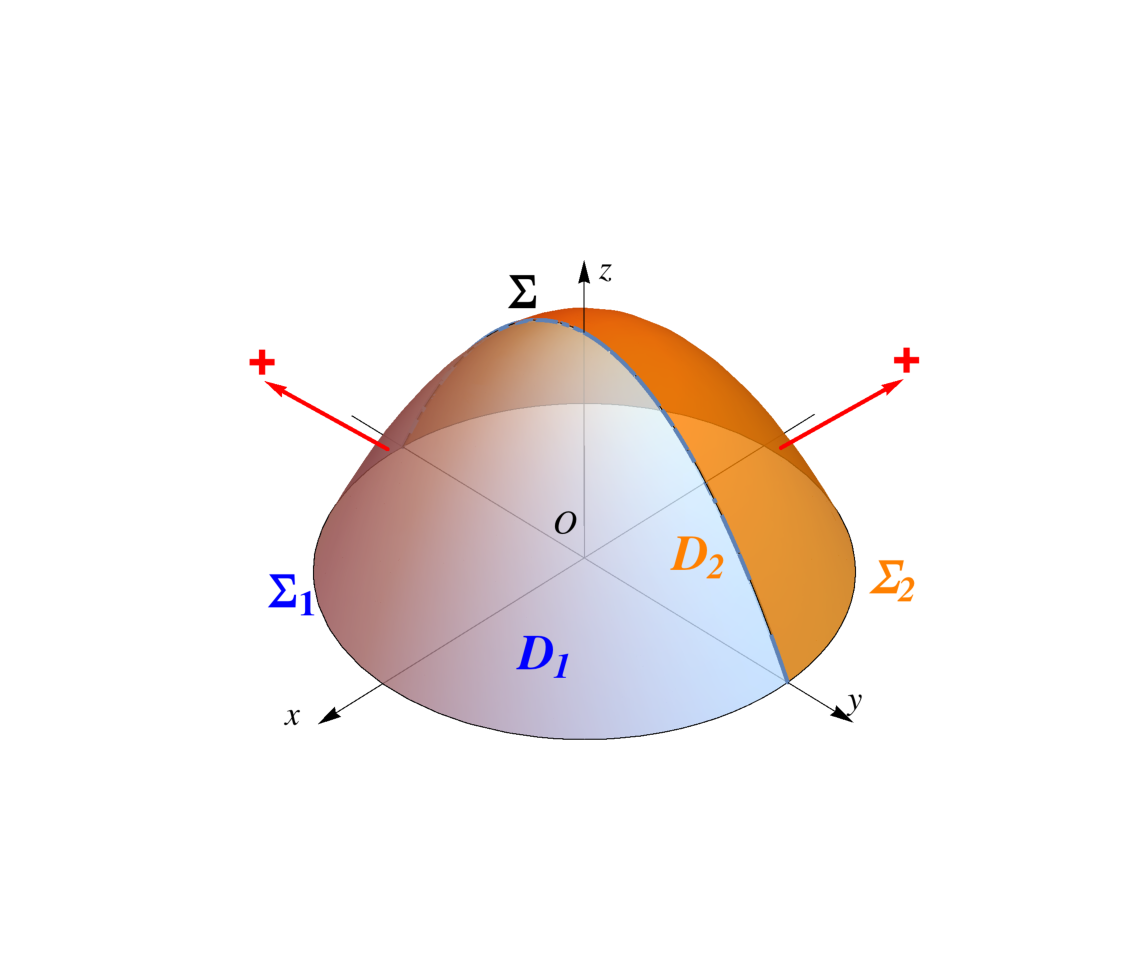
\includegraphics{./images/ch12/xdxy.pdf}}
% \end{center}
% 
% 已知$\Sigma$关于$x=0$对称,$\Sigma_1$和$\Sigma_2$分别为其中对应于
% $x\geq0$和$x\leq0$的部分,$D_1$和$D_2$分别为二者对应的投影。
% 
% 设$\Sigma$的方程为$z=z(x,y),(x,y)\in D_1+D_2$,则由已知,
% $$z(-x,y)=z(x,y).$$
% 设$f(x,y,z)$关于$x$为偶函数,即
% $$f(-x,y,z)=f(x,y,z).$$
% 注意到$\Sigma_1$和$\Sigma_2$的正向与$z$轴正向夹角一致(均为锐角或
% 均为钝角),于是
% 
% \begin{align*}
% 	\iint\limits_{\Sigma_2}&f(x,y,z)\d x\d y
% 	=\iint\limits_{D_2}f(x,y,z(x,y))\d\sigma_{xy}
% 	=\iint\limits_{D_2}f(-x,y,z(-x,y))\d\sigma_{xy}\\
% 	&=\iint\limits_{D_2}f(-x,y,z(-x,y))\d\sigma_{xy}
% 	\xlongequal{u=-x\atop{v=y}}\iint\limits_{D_1}f(u,v,z(u,v))\d\sigma_{uv}\\
% 	&=\iint\limits_{D_1}f(x,y,z(x,y))\d\sigma_{xy}
% 	=\iint\limits_{\Sigma_1}f(x,y,z)\d x\d y
% \end{align*}
% 即证。

例如:$\ds\oiint\limits_{x^2+y^2+z^2=R^2}\df{x}{x^2+3y^2+1}\d x\d y=0$

{\it\color{red} 被积函数关于$z$为奇(偶)函数}:空间曲面{\color{red}$\Sigma$关于$z=0$对称},
$\Sigma_1$为其中$z\geq 0$的部分,则
$${\color{red}\iint\limits_{\Sigma}f(x,y,z)\d x\d y=\left\{\begin{array}{ll}
0,& f(x,y,z)\mbox{关于}z\mbox{是偶函数}\\
2\ds\iint\limits_{\Sigma_1}f(x,y,z)\d x\d y,& f(x,y,z)\mbox{关于}z\mbox{是奇函数}
\end{array}\right.}$$

例如:$\ds\oiint\limits_{x^2+y^2+z^2=R^2}\df{z^2}{x^2+3y^2+1}\d x\d y=0$

例如:设$\Sigma$为$x^2+y^2=R^2$及平面$z=\pm R\,(R>0)$所围立体的外表面,则
$$\oiint\limits_{\Sigma}\df{x\d y\d z+y^2\d z\d x+z^2\d x\d y}{x^2+y^2+z^2}
=\oiint\limits_{\Sigma}\df{x\d y\d z}{x^2+y^2+z^2}$$

{\bf (2)轮换对称}

{\it\color{red} $x,y$的轮换}:\ps{\color{red}
对这里所考虑的积分,任何时候都不可以考虑$x,z$和$y,z$的交换}
{\color{red} 若$\Sigma$中$x,y$地位相同,则在积分
$\iint\limits_{\Sigma}f(x,y,z)\d x\d y$
中$x,y$可交换位置},也即
$$\iint\limits_{\Sigma}f(x,y,z)\d x\d y=\iint\limits_{\Sigma}f(y, x,z)\d x\d y$$

\newpage

\section*{补充习题}

{\bf 例:}设$L$是摆线$x=t-\sin t-\pi,y=1-\cos t$从$t=0$
到$t=2\pi$的一段,则$\dint_L\df{(x-y)\d x+(x+y)\d y}{x^2+y^2}=-\pi$

[提示]:添加路径$L_1:x^2+y^2=\pi^2,\;y\geq 0$,使用Green公式计算。
注意,不能使用路径$y=0$,因为被积函数在原点处无定义!

{\bf 例:}设$L_1:\df{x^2}{4}+\df{y^2}{9}=1,L_2:\df{x^2}{9}+\df{y^2}{4}=1$,
二者所围封闭区域分别为$D_1,D_2$,则下列正确的是\;
(C)
%  		  \vspace{-1cm}
\begin{enumerate}[(A)]
  \item $\dint_{L_1}(x+y^2)\d s=2\dint_{L_2}y^2\d s$
  \item $\dint_{L_1}(x^2+y)\d s=2\dint_{L_2}(x^2+y)\d s$
  \item $\ds\iint_{D_1}(x+y^3)\d\sigma=2\ds\iint_{D_2}(x+y^3)\d\sigma$
  \item $\ds\iint_{D_1}(x^2+y)\d\sigma=2\ds\iint_{D_2}(x^2+y)\d\sigma$
\end{enumerate}

{\bf 例:}$f(x,y)$偏导连续,曲线$L:f(x,y)=1$过第二象限的点$M$
  和第四象限的点$N$,$\Gamma$为$L$上从$M$到$N$的一段弧,则下列
  小于零的是\;
(B)
  \begin{enumerate}[(A)]
  \setlength{\itemindent}{1cm}
    \item $\dint_{\Gamma}f(x,y)\d x$
    \item $\dint_{\Gamma}f(x,y)\d y$
    \item $\ds\int_{\Gamma}f(x,y)\d s$
    \item $\ds\int_{\Gamma}f\,'_x(x,y)\d x+f\,'_y(x,y)\d y$
  \end{enumerate}

{\bf 例:}设曲面$S_1:x^2+y^2+z^2=1(z\geq
  0)$,$S_2$为$S_1$在第一卦限中的部分,
  则以下正确的是\;
  (C) 
  \begin{enumerate}[(A)]
  \setlength{\itemindent}{1cm}
    \item $\ds\iint_{S_1}x\d S=4\iint_{S_2}x\d S$
    \item $\ds\iint_{S_1}y\d S=4\iint_{S_2}x\d S$
    \item $\ds\iint_{S_1}z\d S=4\iint_{S_2}x\d S$
    \item $\ds\iint_{S_1}xyz\d S=4\iint_{S_2}xyz\d S$
  \end{enumerate}

{\bf 例:}设$f(r)$二阶连续可微,$r=\sqrt{x^2+y^2+z^2}$,
  若$\mathrm{div}(\bigtriangledown\,f(r))=0$,则$f(r)=$\;
  (B) 
  \begin{enumerate}[(A)]
  \setlength{\itemindent}{1cm}
    \item $C_1r+C_2$
    \item $C_1/r+C_2$
    \item $C_1r^2+C_2$
    \item $C_1/r^2+C_2$
  \end{enumerate}
  以上$C_1,C_2$为任意常数

{\bf 注:}$\mathrm{div}(\bigtriangledown\,u)=u''_{xx}+u''_{yy}+u''_{zz}$

{\bf 例:}计算第一型曲线积分(设$a>0$)
\begin{enumerate}[(1)]
  \setlength{\itemindent}{1cm}
  \item $\ds\int\limits_{x^{2/3}+y^{2/3}=a^{2/3}}
  \left(x^{4/3}+y^{4/3}\right)\d s$
  \item $\ds\int\limits_{(x^2+y^2)^2=a^2(x^2-y^2)}|y|\d s$
  \item $\ds\int_Cz\d s$
  其中$C$为$x^2+y^2=z^2$与$y^2=ax$的交线上从原点到$(a,a,\sqrt2a)$的一段
\end{enumerate}

[提示]:(1)令$x=a\cos^3t,y=a\sin^3t,t\in[0,2\pi]$

(2)曲线的极坐标方程:$\rho=a\sqrt{\cos2\theta},\theta\in\left[-\df{\pi}4,
\df{\pi}4\right]\cup\left[\df{3\pi}4,\df{5\pi}4\right]$,然后利用
$$\d s=\sqrt{\rho^2+(\rho')^2}\d\theta$$
计算弧长微元

(3)以$y$为参数建立曲线的参数方程。

{\bf 例:}计算积分
$$I=\int_Ly^2\d x+z^2\d y+x^2\d z,$$
其中$C$为曲线$\left\{\begin{array}{l}
x^2+y^2+z^2=1 \\ x^2+y^2=x
\end{array}\right.$
上$z\geq 0$的部分,从$x$轴正向看去为逆时针方向。

[提示]:方法一:直接计算,曲线的参数方程为 
$$x=\cos^2\theta,y=a\cos\theta\sin\theta, z=a|\sin\theta|\;
(\theta\in[-\pi/2,\pi/2])$$

方法二:Stokes公式。

{\bf 例:}设$L$为平面上的简单光滑闭曲线,$D$为$L$所围成的有界闭区域,$\bm{n}$
为$L$的外法向,$\df{\p u}{\p\bm{n}}$表示函数$u(x,y)$沿$\bm{n}$的方向导数
\begin{enumerate}[(1)]
  \setlength{\itemindent}{1cm}
  \item 将$\ds\oint_L\df{\p u}{\p\bm{n}}\d s$化为对坐标的曲线积分;
  \item 设$u=x^2+y^2$,$L:x^2+y^2=6x$,计算
  $$\ds\oint_L\df{\p u}{\p\bm{n}}\d s$$
\end{enumerate}

[提示]:辅导书-P137-例3

{\bf 例:}设$f(x)$当$x>0$时可导,$f(1)=2$,对右半平面内的任意封闭曲线$C$,
有$\ds\oint_C4x^3y\d x+xf(x)\d y=0$
\begin{enumerate}[(1)]
  \setlength{\itemindent}{1cm}
  \item 求$f(x)$;
  \item 设$L$为从$(1,0)$到$(2,3)$的一段弧,计算
  $$\dint_L4x^3y\d x+xf(x)\d y$$
\end{enumerate}

[提示]:由全微分方程的条件,得到关于$f(x)$的微分方程,可解得$f(x)=\df{x^4+1}x$

{\bf 例:}已知曲线$L:\left\{\begin{array}{l}
	x^2+y^2+z^2=R^2\\ x+y+z=0
\end{array}\right.$,
计算曲线积分
$$\oint_Lz^2\d s$$

[提示]:利用轮换对称性
$$\oint_Lz^2\d s=\df13\oint_L(x^2+y^2+z^2)\d s
=\df13\oint_LR^2\d s=\df23\pi R^3.$$

{\bf 例:}函数$u(x,y),v(x,y)$在单位圆内存在一阶连续偏导数,
$$\bm{f}(x,y)=(v(x,y),u(x,y)),$$
$$\bm{g}(x,y)=\left(u'_x-u'_y,v'_x-v'_y\right),$$
在单位圆上,$u(x,y)=x,v(x,y)=1$,求
$$\iint_{x^2+y^2\leq 1}\bm{f}\cdot\bm{g}\d\sigma$$

[提示]:
\begin{align}
	&\iint\limits_{x^2+y^2\leq 1}\bm{f}\cdot\bm{g}\d\sigma\notag
    =\iint\limits_{x^2+y^2\leq 1}\left[(vu'_x+uv'_x)-
	(vu'_y+uv'_y)\right]\d\sigma\notag\\
	&=\iint\limits_{x^2+y^2\leq 1}\left[(uv)'_x-(uv)'_y\right]
	\d\sigma\notag\\
	&=\oint_{x^2+y^2=1}(uv)\d x+(uv)\d y
	=\oint_{x^2+y^2=1}x\d x+x\d y\notag\\
	&=\iint\limits_{x^2+y^2\leq 1}\d\sigma=\pi\notag
\end{align}

{\bf 例:}在变力$\bm{F}=(yz,zx,xy)$的作用下,质点由原点沿直线运动到椭球面
$\df{x^2}{a^2}+\df{y^2}{b^2}+\df{z^2}{c^2}=1$上第一卦限
中的某点$M$,问$M$在何位置时,$\bm{F}$所做的功最大,并求出功的最大值。

[提示]:首先验证$\bm{F}$为保守场,再根据$M$在椭球面的位置,求功的最大值

\section{小结}

能够正确理解这张图里每个概念和公式,这张应该就没什么大问题了,嘿\ldots

\bigskip

\tikzstyle{int}=[ultra thick, rounded corners,
	draw=black!40,fill=red!10!white,
 	inner sep=1ex,
	text width=2.5cm,
% 	text height=5ex,
	minimum height=1.8cm,
	text centered]
\tikzstyle{mint}=[ultra thick, rounded corners,
	draw=black!40,fill=yellow!10!green!10,
 	inner sep=1ex,
	minimum width=3.5cm,
% 	text height=5ex,
	minimum height=1.5cm,
	text centered]
\tikzstyle{arrow}=[thick,blue!80]
\begin{tikzpicture}
 	[node distance=4cm, >=stealth', thick, bend angle=45, auto]
	\node [int] (iiint) 
		{\large 三重积分\\
		\small$\ds\iiint\limits_{\Omega}f(x,y,z)\d V$
	};
	\node [int, below of=iiint] (iint) 
		{\large 二重积分\\
		\small$\ds\iint\limits_Df(x,y)\d\sigma$
	};
	\node [int, below of=iint] (int) 
		{\large 定积分\\
		\small$\ds\int_a^bf(x)\d x$
	};
	\node [mint, right of = int, xshift=2.5cm] (NL)
% 		{\color{red}Netwon-Lebniz\it 公式};
		{\small $\dint_A^Bf(\bm{x})\d\bm{x}=F(\bm{x})|_A^B$};
% 	\node [right of = int, xshift = 3cm, minimum width=5cm,
% 		minimum height = 1.5cm] (NL)
% 		{\small$\ds\int_a^bf(x)\d x=F(b)-F(a)$};
	\begin{scope}[xshift=5.5cm]
		\node [int] (sint) 
			{\large 曲面积分
			};
		\node [int, below of = sint] (cint)
			{\large 曲线积分
			};
	\end{scope}
	\begin{scope}[xshift=11cm,yshift=1.6cm]
		\node [mint] (sint1) 
			{\small$\ds\iint\limits_{\Sigma}f(x,y,z)\d S$};
		\node [mint, below of = sint1, yshift=1.5cm] (sint2)
			{\small$\ds\iint\limits_{\Sigma}f(x,y,z)\d x\d y$};
		\node [mint, below of = sint2, yshift=2cm] (cint1)
			{\small$\ds\int_Lf(\bm{x})\d s$};
		\node [mint, below of = cint1, yshift=1.5cm] (cint2)
			{\small$\ds\int_LP\d x+Q\d y+R\d z$};
	\end{scope}
	\path (iiint) edge[arrow,<->]
		node [text width=3em]{\it 柱坐标 球坐标} 
		node[swap, text width=3em,text centered] {“1+2”  “2+1”} (iint)
		edge[arrow,<->] 
		node {\color{red}Gauss\it 公式}(sint);
	\path (iint) edge[arrow,<->] 
		node[swap, text width=3em,text centered] {“1+1”  \it 定限} 
		node[text width=4em] {\it 极坐标} (int)
		edge[arrow,<->] 
		node {\color{red}Green\it 公式} (cint);
	\path (sint) edge [arrow,->] 
		node [sloped,pos=0.2,swap]{\it 投影/曲面方程}(iint)
		edge[arrow,<->] 
		node {\color{red}Stokes\it 公式}(cint)
		edge[arrow] node[sloped,pos=0.8]{\it 对面积} (sint1)
		edge[arrow] node[sloped,pos=0.2]{\it 对坐标}(sint2);
	\path (cint) edge [arrow, ->] 
		node [sloped,near start,swap]{\it 曲线参数化} (int)
		edge [arrow] node[sloped,pos=0.8]{\it 对弧长}(cint1)
		edge [arrow] node[sloped,pos=0.2]{\it 对坐标}(cint2);
	\path (sint1) edge[arrow, <->] 
		node {\color{red}$\d\sigma_{xy}=|\cos\gamma|\d S$} (sint2);
	\path (cint1) edge[arrow, <->] 
		node {\color{red}$\d s=|\bm{r}'(t)|\d t$} (cint2);
	\path (cint2) edge [arrow, ->, out=-90, in=0, dashed] 
		node {\it 积分与路径无关条件} (NL);
	\path (int) edge [arrow, ->, dashed]
		node {{\color{red}Netwon-Lebniz}}
		node [swap]{\color{red}\it 公式} (NL);
% 	\path (int) edge[<->] (NL);
\end{tikzpicture}

\newpage

\section*{课后作业}
\addcontentsline{toc}{section}{课后作业}

{\bf 【必作题】}

\begin{itemize}
  \setlength{\itemindent}{1cm}
  \item 习题12.1:8,10(1,3),11,13,15,16(2),18,21
  \item 习题12.2:4,8,9,12,15,18,19
  \item 习题12.3:2(1),3,6,9,11,13,15,19
  \item 习题12.4:3(2),4,8(2,4),9,10,14
\end{itemize}

\bigskip

\hrule

\bigskip

{\bf 【思考题】}

1.\;设$L$为曲线$x=\df{3at}{1+t^3},y=\df{3at^2}{1+t^3}$上$t$由
$0$到$+\infty$的一段,$a>0$,求$\dint_Lx\d y-y\d x$

2.\;$f(x)$连续可导,$L$为$(3,2/3)$到$(1,2)$的直线,
求$\dint_L\df{1+y^2f(xy)}y\d x+\df x{y^2}[y^2f(xy)-1]\d y$

3.\;计算$\ds\iint\limits_{z=\sqrt{a^2-x^2-y^2}}(x+y+z)\d S=\pi a^3$

4.\;设$\Sigma$为平面$x+y+z=1$在第一卦限的上侧,$f(x,y,z)$连续,求
$\ds\iint_{\Sigma}[f(x,y,z)+x]\d y\d z-[2f(x,y,z)-y]\d z\d x+
[f(x,y,z)+z]\d x\d y$

5.\;设$f(x)$当$x>0$时可导,$f(1)=2$,对右半平面内的任意封闭曲线$C$,
有$\ds\oint_C4x^3y\d x+xf(x)\d y=0$,求$f(x)$。

6.\;函数$u(x,y),v(x,y)$在单位圆内存在一阶连续偏导数,
$$\bm{f}(x,y)=(v(x,y),u(x,y)),$$
$$\bm{g}(x,y)=\left(u'_x-u'_y,v'_x-v'_y\right),$$
在单位圆上,$u(x,y)=x,v(x,y)=1$,求
$$\iint\limits_{x^2+y^2\leq 1}\bm{f}\cdot\bm{g}\d\sigma$$

7.\;设$\Sigma$为曲面$z=\sqrt{x^2+y^2}$及平面$z=1$和$z=2$
所围立体的外表面,求
$$\oiint\limits_{\Sigma}\sqrt{x^2+y^2}e^z(\d y\d z+\d z\d x+\d x\d y)$$

8.\;设$\Sigma$为$x^2+y^2=R^2$及平面$z=\pm R\,(R>0)$所围立体的外表面,求
$$\oiint\limits_{\Sigma}\df{x\d y\d z+y^2\d z\d x+z^2\d x\d y}{x^2+y^2+z^2}$$

9.\;设$\Sigma$为$2x^2+2y^2+z^2=4$的外侧,求
$$\oiint\limits_{\Sigma}\df{x\d y\d z+y\d z\d x+z\d x\d
y}{(x^2+y^2+z^2)^{3/2}}$$

10.\;在变力$\bm{F}=(yz,zx,xy)$的作用下,质点由原点沿直线运动到椭球面
$\df{x^2}{a^2}+\df{y^2}{b^2}+\df{z^2}{c^2}=1$上第一卦限
中的某点$M$,问$M$在何位置时,$\bm{F}$所做的功最大,并求出功的最大值。


\newpage

% \visibletrue

\ifvisible

\setcounter{section}{1}

\section{Green公式及其应用}

\begin{shaded}
% 	\centerline{\bf 背景资料}
	George Green (1793-1841) , 英国数学与物理学家,生于英国Nottingham,
	自学(只上过一年小学)成才,1828年发表《论应用数学分析于电磁学》
	({\it An Essay on the Application of Mathematical Analysis to 
	the Theories of Electricity and Magnetism }(Green, 1828));
	1833年(40岁)进入Cambridge University学习,1837年毕业后留在剑桥
	冈维尔与凯斯学院。格林在世时,他的工作在数学界并不知名。但到了公元1846年,
	物理学家Lord Kelvin(开尔文勋爵,William Thomson, 1st Baron 
	Kelvin)重新发现了格林的著作,将其推广给后来的数学家。
	
	\bigskip

	1993年,Westminster Abbey设置了纪念George Green的石碑,
	紧邻Sir Isaac Newton 和Lord Kelvin。
	
	\bigskip
	
	Nottingham Review's obituary to George Green:
	
	{\it ... we believe he was the son of a miller, residing near 
	Nottingham, but having a taste for study, he applied his 
	gifted mind to the science of mathematics, in which he 
	made a rapid progress. In Sir Edward Ffrench Bromhead, 
	Bart., he found a warm friend, and to his influence he 
	owed much, while studying at Cambridge. Had his life been 
	prolonged, he might have stood eminently high as a mathematician.}
	
	\hfill (from: http://www-history.mcs.st-and.ac.uk/Biographies/Green.html)
	
	\bigskip
	
	{\it Green pioneered the application of mathematics to physical 
	problems and theorems derived from his work on electricity 
	and magnetism are used in modern nuclear and solid state physics.}
	
	\hfill (http://www.westminster-abbey.org/our-history/people/george-green)
	
	\bigskip
	
	{\it Green was the first person to create a mathematical theory 
	of electricity and magnetism and his theory formed the foundation 
	for the work of other scientists such as James Clerk Maxwell, 
	William Thomson, and others. His work on potential theory ran 
	parallel to that of Carl Friedrich Gauss.}
	
	\hfill (http://en.wikipedia.org/wiki/George\_Green\_(mathematician))
% 	{\begin{lstlisting}[language=html]
% 		http://en.wikipedia.org/wiki/George_Green_(mathematician)
% 	\end{lstlisting}}
	
	\bigskip
	
	Green公式在物理上的意义就是闭合曲线Γ内所有微环流量(Microscopic circulation)
	的总和等于沿曲线Γ方向的线积分(Macroscopic circulation)。

	\hfill (http://www.cnblogs.com/frischzenger/archive/
	2009/06/15/1503819.html)

	\bigskip
	Green公式的几何意义,童志通,《数学通报》 1965年07期 加入收藏 投稿
\end{shaded}

{\bf 定理12.2.1-3:}$$\oint_LP(x,y)\d x+Q(x,y)\d y=\iint_D\left(
\df{\p Q}{\p x}-\df{\p P}{\p y}\right)\d\sigma$$

\begin{enumerate}[(1)]
  \setlength{\itemindent}{1cm}
  \item $D$:$xOy$平面内的有界闭区域
  \item $L=\p D$:分段光滑曲线,按{\it “左侧法则”}取正向
  \item $P(x,y),Q(x,y)$在$D$内有连续偏导数
\end{enumerate}

[证明思路]:先证:$\ds\oint_LQ(x,y)\d y=\ds\iint_D\df{\p Q}{\p x}\d\sigma$。
\begin{center}
	\resizebox{!}{5cm}{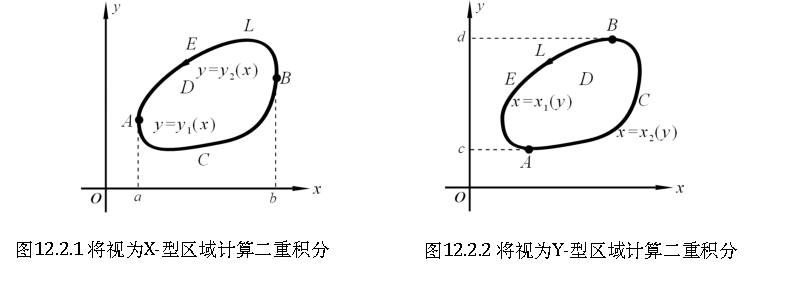
\includegraphics{./images/ch12/xy-Green.pdf}}
\end{center}
事实上,如图12.2.2,区域$D$可以表示为
$$D:y_1\leq y\leq y_2,\;x_1(y)\leq x\leq x_2(y).$$
故
\begin{eqnarray*}
	\mbox{右边}&=&\dint_{y_1}^{y_2}\dint_{x_1(y)}^{x_2(y)}
	Q'_y(x,y)\d x\d y\\
	&=&\dint_{y_1}^{y_2}\left.Q(x,y)\right|_{x_1(y)}^{x_2(y)}\d y\\
	&=&\dint_{y_1}^{y_2}\left[Q(x_2(y),y)-Q(x_1(y),y)\right]\d y
\end{eqnarray*}
又$L=L_1+L_2$,故
\begin{eqnarray*}
	\mbox{左边}&=&\left(\dint_{L_1}+\dint_{L_2}\right)Q(x,y)\d y\\
	&=&\dint_{y_2}^{y_1}Q(x_1(y),y)\d y+\dint_{y_1}^{y_2}Q(x_2(y),y)\d y\\
	&=&\mbox{右边}
\end{eqnarray*}

同理,可以证明:$\ds\oint_LP(x,y)\d x=-\ds\iint_D\df{\p P}{\p y}\d\sigma$。

{\bf 思考:}为什么两个部分存在符号上的差异?({\it 因为曲线靠近$x,y$的部分的方向与两个
坐标轴的相对方向不同!})


{\bf 例:}计算曲线积分$\dint_Lx\d y-y\d x$,其中$L:\df{x^2}{a^2}+\df{y^2}{b^2}=1$
取逆时针方向。

[提示]:由Green公式
$$\dint_Lx\d y-y\d x=2\iint_D\d\sigma=2\pi ab.$$
事实上,如果直接计算该曲线积分,令$x=a\cos t,y=b\sin t,t\in[0,2\pi]$,则
$$\dint_Lx\d y-y\d x=\dint_0^{2\pi}a\cos t\d(b\sin t)
-b\sin t\d(a\cos t)=ab\dint_0^{2\pi}\d t=2\pi ab.$$

{\bf 注:}该公式可以作为求给定平面区域面积的一种方法,适用于任意边界为分段光滑曲线
的有界闭区域,即
$$S_D=\iint_D\d\sigma=\df12\oint_{\p D}x\d y-y\d x$$

{\bf 关于Green公式的讨论:}
\begin{enumerate}[(1)]
  \setlength{\itemindent}{1cm}
  \item $L$可以包含平行于$x$轴和$y$轴的直线
  \item $D$可以是简单闭区域、单连通域或多连通域
\end{enumerate}

\begin{center}
	\resizebox{!}{10cm}{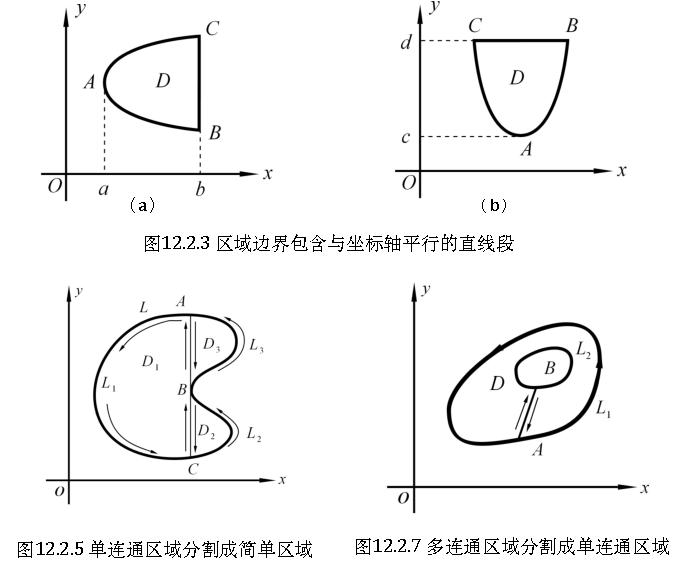
\includegraphics{./images/ch12/d-k.pdf}}
\end{center}

如图12.2.5,
\begin{eqnarray*}
	\iint_D\left(\df{\p Q}{\p x}-\df{\p P}{\p y}\right)\d\sigma&=&
	\left(\iint_{D_1}+\iint_{D_2}+\iint_{D_3}\right)\left(\df{\p Q}{\p x}-\df{\p
	P}{\p y}\right)\d\sigma\\
	&=&\left(\oint_{L_1}+\oint_{L_2}+\oint_{L_3}\right)P\d x+Q\d y\\
	&=&\oint_LP\d x+Q\d y
\end{eqnarray*}

% \begin{shaded}
% 	\centerline{\bf 用差分化方法求曲线积分}
% % 	\begin{tabularx}{\textwidth}{XX}
% % 		\resizebox{!}{6.5cm}{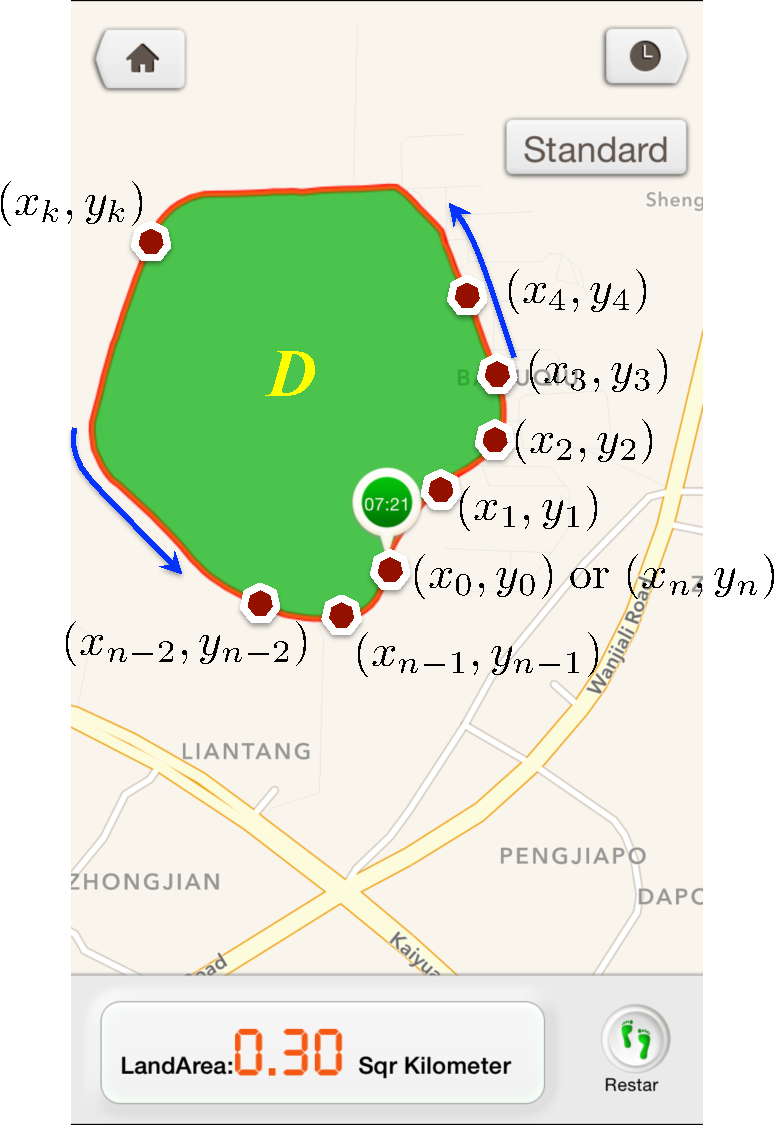
\includegraphics{./images/ch12/YCSam.pdf}}
% % 		&
% % 		$$\ds\iint_D\d\sigma=\df12\ds\oint_Lx\d y-y\d x
% % 		\approx\df12\sum\limits_{k=1}^n$$
% % 		其中
% % 		\begin{itemize}
% % 		  \item $(x_k,y_k)\;(k=0,1,2,\ldots,n)$:GPS采样点 
% % 		  \item $\Delta x_k=x_k-x_{k-1},k=1,2,\ldots,n$ 
% % 		  \item $\Delta y_k=y_k-y_{k-1},\;k=1,2,\ldots,n$
% % 		\end{itemize}
% % 	\end{tabularx}
% % 	\begin{tabular}{cl}
% % 		\resizebox{!}{6.5cm}{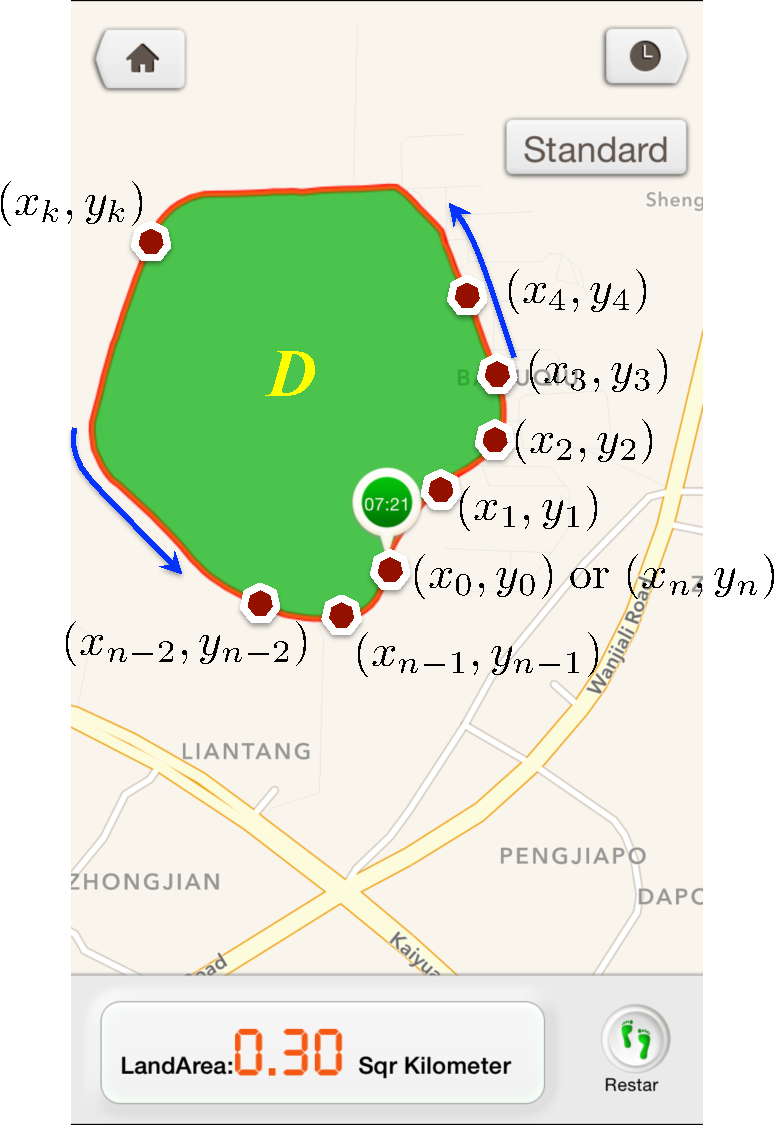
\includegraphics{./images/ch12/YCSam.pdf}}
% % 		&
% % 		$$\ds\iint_D\d\sigma=\df12\ds\oint_Lx\d y-y\d x
% % 		\approx\df12\sum\limits_{k=1}^n$$
% % 		其中
% % 		\begin{itemize}
% % 		  \item $(x_k,y_k)\;(k=0,1,2,\ldots,n)$:GPS采样点
% % 		  \item $\Delta x_k=x_k-x_{k-1},k=1,2,\ldots,n$
% % 		  \item $\Delta y_k=y_k-y_{k-1},\;k=1,2,\ldots,n$
% % 		\end{itemize}
% % 	\end{tabular}
% 	
% % 	$$\ds\iint_D\d\sigma=\df12\ds\oint_Lx\d y-y\d x
% % 	\approx\df12\sum\limits_{k=1}^n$$
% % 	其中
% % 	\begin{itemize}
% % 	  \item $(x_k,y_k)\;(k=0,1,2,\ldots,n)$:GPS采样点
% % 	  \item $\Delta x_k=x_k-x_{k-1},k=1,2,\ldots,n$
% % 	  \item $\Delta y_k=y_k-y_{k-1},\;k=1,2,\ldots,n$
% % 	\end{itemize}
% % 	\begin{center}
% % 		\resizebox{!}{6.5cm}{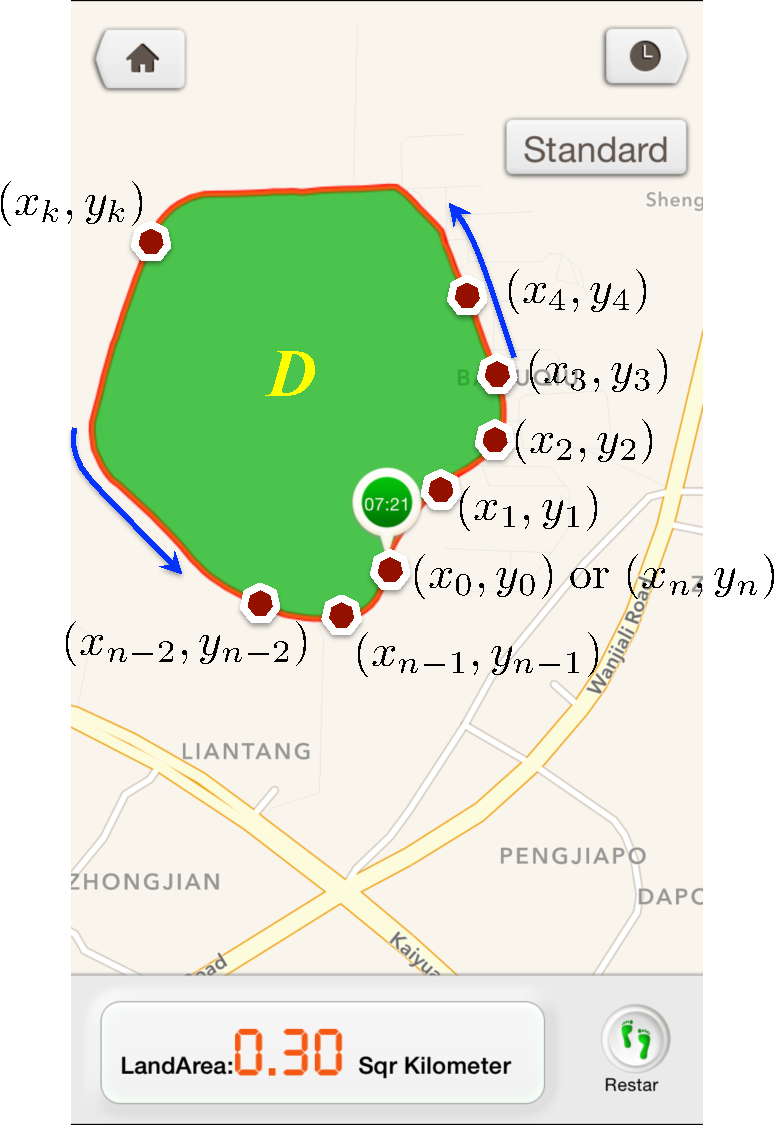
\includegraphics{./images/ch12/YCSam.pdf}}
% % 	\end{center}
% 	
% 	\begin{figure}[htbp]%
% 		\centering
% 		\begin{minipage}[b]{0.4\textwidth}
% 			\centering
% 			\resizebox{!}{7cm}{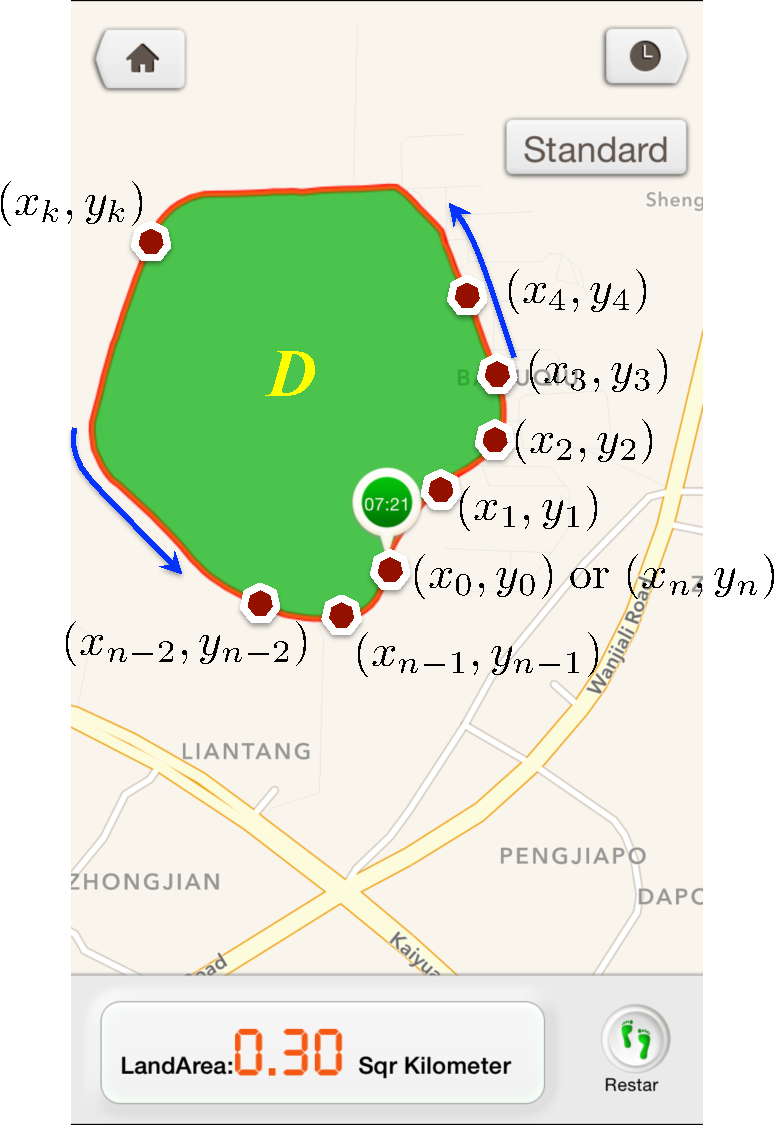
\includegraphics{./images/ch12/YCSam.pdf}}
% 	% 		\caption{清明}
% 		\end{minipage}
% 		\begin{minipage}[b]{0.5\textwidth}
% 			$$\ds\iint_D\d\sigma=\df12\ds\oint_Lx\d y-y\d x
% 			\approx\df12\sum\limits_{k=1}^n$$
% 			其中
% 			\begin{itemize}
% 			  \item $(x_k,y_k)\;(k=0,1,2,\ldots,n)$:GPS采样点
% 			  \item $\Delta x_k=x_k-x_{k-1},k=1,2,\ldots,n$
% 			  \item $\Delta y_k=y_k-y_{k-1},\;k=1,2,\ldots,n$
% 			\end{itemize}
% 		\end{minipage}
% 	\end{figure}
% \end{shaded}

\bigskip

\hrule

\bigskip

\begin{figure}[htbp]%
	\centering
	\begin{minipage}{0.4\textwidth}
		\centering
		\resizebox{!}{7cm}{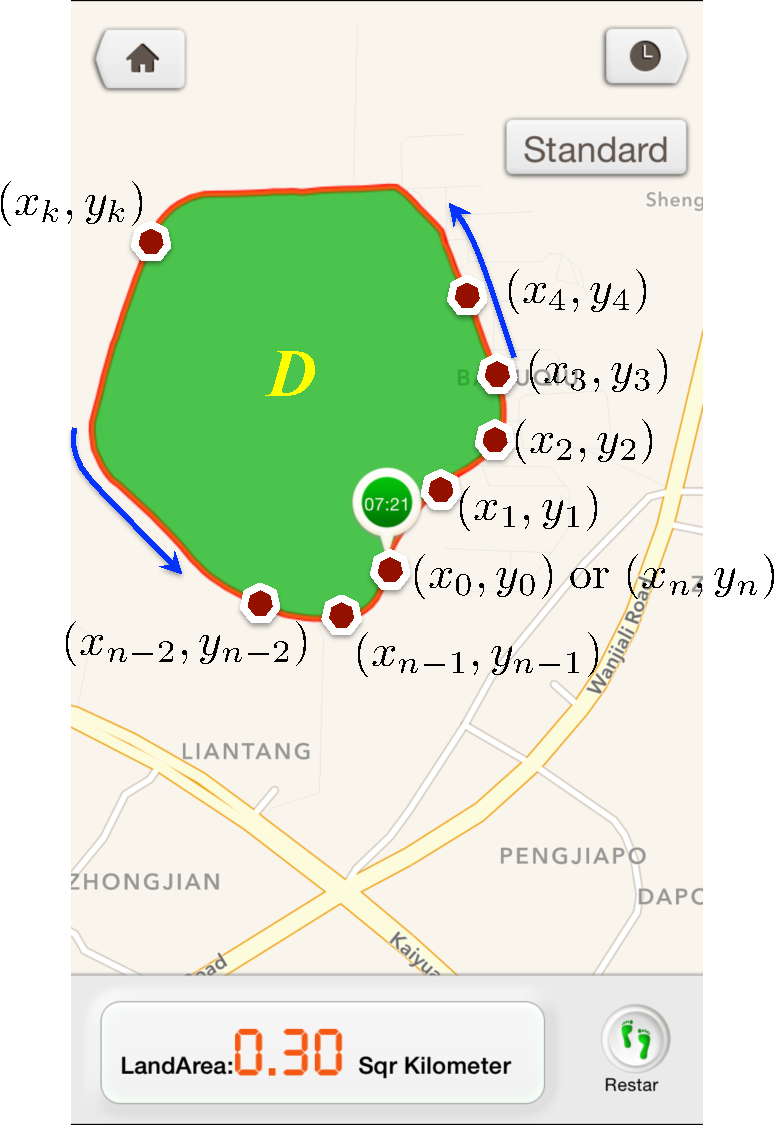
\includegraphics{./images/ch12/YCSam.pdf}}
% 		\caption{清明}
	\end{minipage}
	\begin{minipage}{0.5\textwidth}
		{\bf 用差分化方法求曲线积分}
		\begin{eqnarray*}
			\ds\iint_D\d\sigma&=&\df12\ds\oint_Lx\d y-y\d x\\
			&\approx&\df12\sum\limits_{k=1}^n(x_k\Delta y_k-y_k\Delta x_k)
		\end{eqnarray*}
		其中
		\begin{itemize}
		  \item $(x_k,y_k)\;(k=0,1,2,\ldots,n)$:GPS采样点
		  \item $\Delta x_k=x_k-x_{k-1},k=1,2,\ldots,n$
		  \item $\Delta y_k=y_k-y_{k-1},\;k=1,2,\ldots,n$
		\end{itemize}
	\end{minipage}
\end{figure}

\bigskip

\hrule

\bigskip

{\bf 小结}

\begin{enumerate}[(1)]
  \setlength{\itemindent}{1cm}
  \item Green公式
  	$$\oint_LP\d x+Q\d y=\iint_D\left(
	\df{\p Q}{\p x}-\df{\p P}{\p y}\right)\d\sigma$$
	\begin{itemize}
	  \item 掌握证明的基本思路
	  \item 正确理解定理条件
	\end{itemize}
  \item 利用Green公式求平面区域面积
    $$\ds\iint_D\d\sigma=\df12\ds\oint_Lx\d y-y\d x$$
\end{enumerate}

{\bf 课后作业:}习题12.2:1,3,4

\bigskip

\hrule

\bigskip

{\bf 课后思考:}查阅关于{\it Planimeter(求积仪)}的资料,结合Green公式
解释其工作原理。

\begin{center}
	\resizebox{!}{7cm}{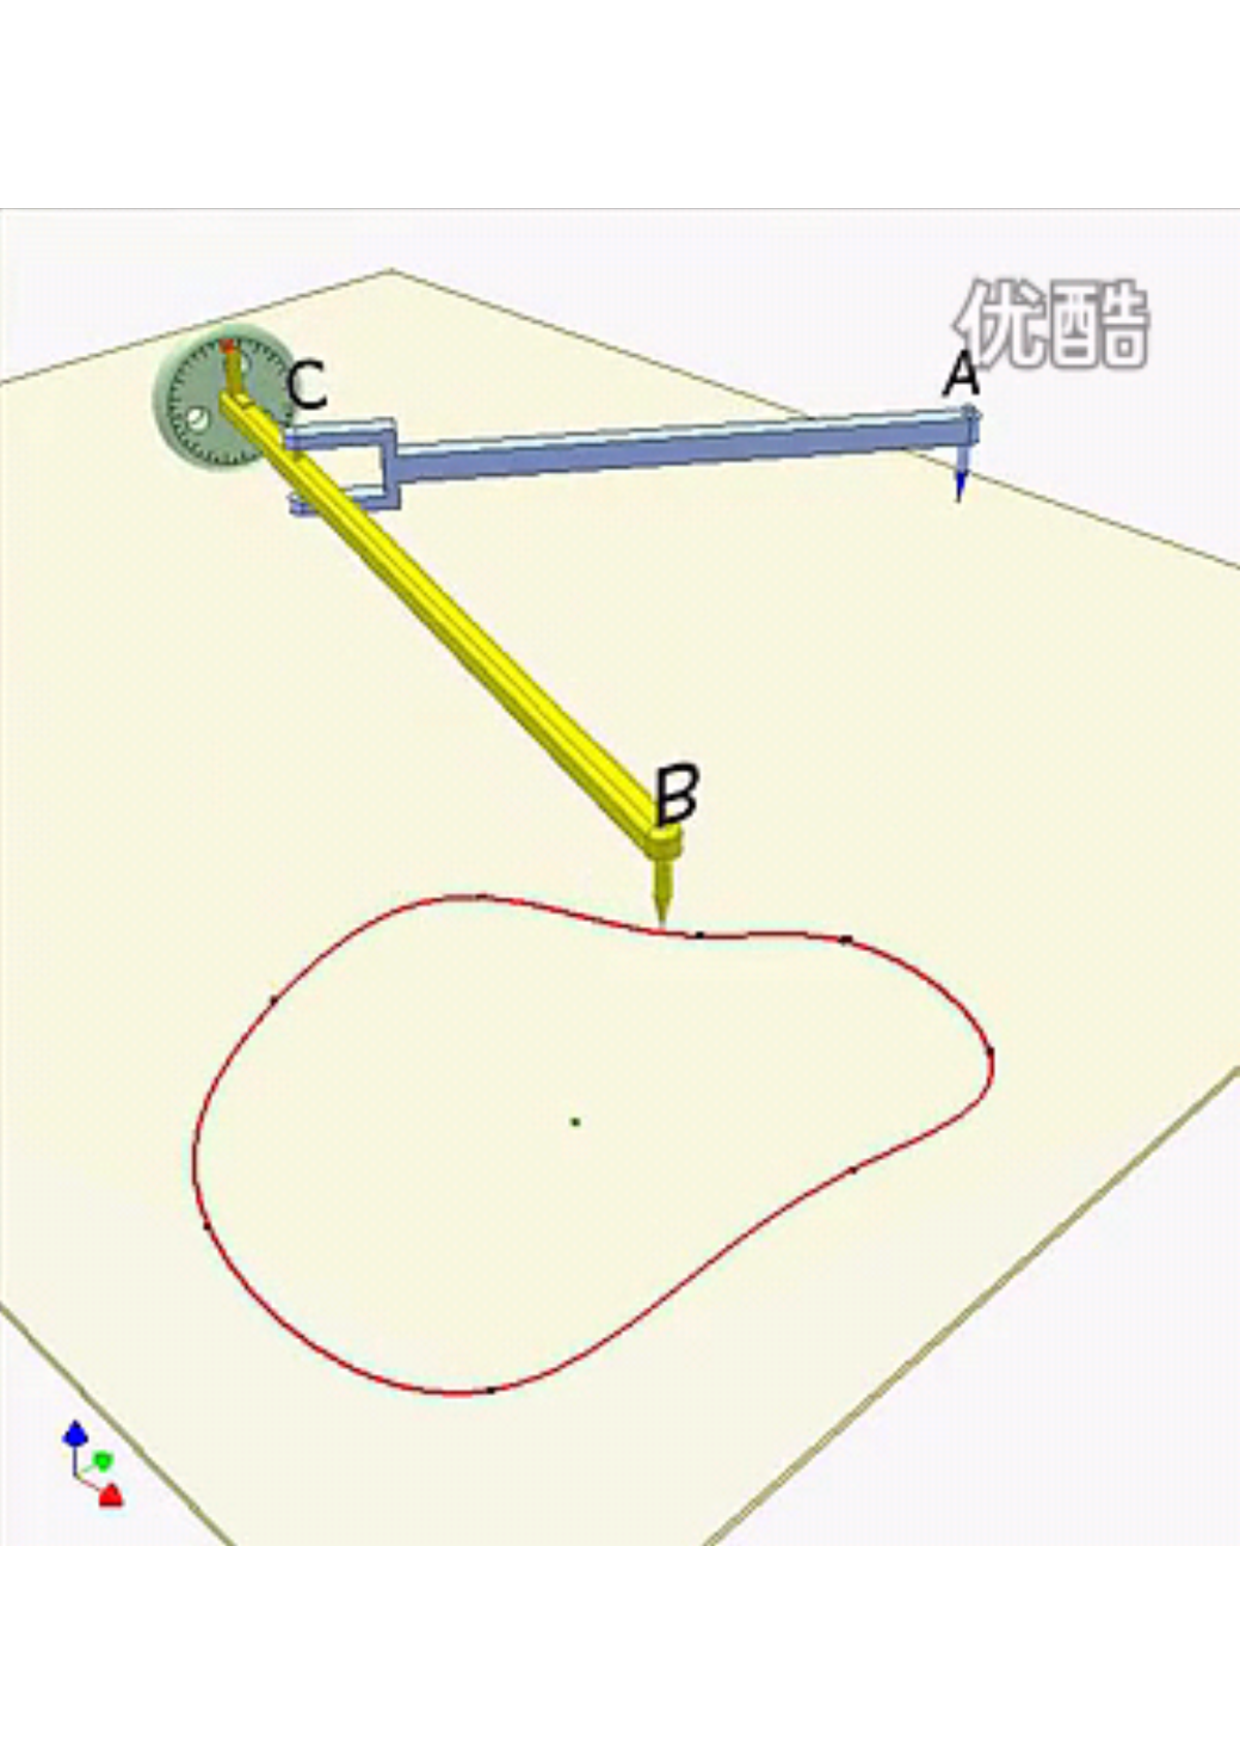
\includegraphics{./images/ch12/planiMeter.pdf}}
	
	(http://v.youku.com/v\_show/id\_XNzIzMDkzMTgw.html?from=s1.8-1-1.2)
\end{center}

\fi

\section*{习题参考解答}
\addcontentsline{toc}{section}{习题参考解答}

\begin{center}
	\bf 11.1 第一型的曲线积分与曲面积分
\end{center}

1.已知$a>0$,计算积分$\dint_L z\d s$,其中$L$为$x^2+y^2=z^2$与$y^2=ax$
的交线上从原点到$(a,a,\sqrt2a)$的一段。

[解]:由曲线方程可求得
$$y'_x=\df{a}{2y},\quad z'_x=\df{2x+a}{2z},\quad x\in[0,a],$$
进而弧长微元可表示为
$$\d s=\sqrt{1+(y'_x)^2+(z'_x)^2}\d x
=\df z2\sqrt{8x^2+9ax+2a^2}\d x,$$
于是
\begin{align*}
	\mbox{原式}&=\dint_0^a\df12\sqrt{8x^2+9ax+2a^2}\d x
	=\df{a^2}{32}(25\sqrt{19}-9\sqrt2)
	+\df{17\sqrt2 a^2}{256}\ln\df{17}{25+4\sqrt{38}}.
\end{align*}
\fin

\bs

2.已知$a>0$,计算积分$\dint_{\Gamma}(x^2+y^2+z^2)\d s$,其中$\Gamma$
为$x^2+y^2=a^2$与$z=1$的交线。

[解]:
\begin{align*}
	\mbox{原式}&=\dint_{\Gamma}(a^2+1)\d s=(a^2+1)\dint_{\Gamma}\d s
	=2\pi a(a^2+1).
\end{align*}
\fin

\bs

3.已知某曲线$L$的线密度为$\mu=x^2+y^2+z^2$,方程为
$$x=e^t\cos\theta,\;y=e^t\sin\theta,\;z=\sqrt2e^t,\;-\infty<t\leq0.$$
求该曲线绕$z$轴转动的转动惯量。

[解]:由已知易得弧长微元
$$\d s=\sqrt3e^t\d t,\quad t\in(-\infty,0],$$
进而
\begin{align*}
	\mbox{原式}
	&=\dint_L(x^2+y^2)\mu\d s
	=\dint_{-\infty}^0e^{2t}(3e^{2t})\sqrt3e^t\d t=\df{3\sqrt3}5.
\end{align*}
\fin

\bs

4.计算积分$\ds\iint_{\Sigma}(x+y+z)\d S$,其中$\Sigma$为半径为
$R$的上半球面。

[解]:注意到$\Sigma$关于$x=0$和$y=0$对称,故
$$\ds\iint_{\Sigma}x\d S=\ds\iint_{\Sigma}y\d S=0,$$
又由上半球面的方程$z=\sqrt{R^2-x^2-y^2}$可得$\d S=\df{R}z\d\sigma_{xy}$,
故
\begin{align*}
	\mbox{原式}&=\ds\iint_{\Sigma}z\d S
	=\ds\iint_{x^2+y^2\leq R^2}z\df{R}z\d\sigma_{xy}
	=R\ds\iint_{x^2+y^2\leq R^2}\d\sigma_{xy}
	=\pi R^3.
\end{align*}
\fin

\bs

5.计算积分$\ds\iint_S x^2\d S$,其中$S$为圆柱面$x^2+y^2=a^2$介于
$z=0$和$z=h$之间的部分。

[解]:注意到$S$中$x,y$是可交换的,故必有
$$\ds\iint_S x^2\d S=\ds\iint_S y^2\d S,$$
从而
\begin{align*}
	\mbox{原式}
	&=\df12\ds\iint_S (x^2+y^2)\d S
	=\df12\ds\iint_S a^2\d S
	=a^2\df12\ds\iint_S \d S=\pi a^3h.
\end{align*}
\fin

\bs

6.计算积分$\ds\iint_{\Sigma}(ax^2+by^2+cz^2)\d S$,其中
$\Sigma$为单位球面。

[解]:注意到在$\Sigma$中$x,y,z$可相互替换,故必有
$$\ds\iint_{\Sigma}x^2\d S=\ds\iint_{\Sigma}y^2\d S
=\ds\iint_{\Sigma}z^2\d S,$$
从而
\begin{align*}
	\mbox{原式}
	&=\df{a+b+c}3\ds\iint_{\Sigma}(x^2+y^2+z^2)\d S
	=\df{a+b+c}3\ds\iint_{\Sigma}\d S=\df{4\pi}3(a+b+c).
\end{align*}
\fin

\bs

7.设球面$x^2+y^2+z^2=2x$的面密度$\mu=x^2+y^2+z^2$,求其质量。

[解]:由已知所求质量
\begin{align*}
	M&=\iint_{\Sigma}\mu\d S=\iint_{\Sigma}(x^2+y^2+z^2)\d S
	=2\iint_{\Sigma}x\d S.
\end{align*}
记上半球面为$\Sigma_1$,则在$\Sigma_1$上$z=\sqrt{1-(x-1)^2-y^2},(x,y)\in D_{xy}$,
其中$D_{xy}:(x-1)^2+y^2\leq 1$。不难得到
$$\d S=\df1z\d\sigma_{xy},$$
从而(以下令$x=1+\rho\cos t,y=\rho\sin t$)
\begin{align*}
	M&=4\iint_{\Sigma_1}x\d S
	=4\iint_{D_{xy}}\df{x}{\sqrt{1-(x-1)^2-y^2}}\d\sigma_{xy}\\
	&=4\dint_0^{2\pi}\dint_0^1\df{1+\rho\cos t}{\sqrt{1-\rho^2}}\rho\d\rho\d t
	=8\pi.
\end{align*}
\fin

\bs

\begin{center}
	\bf 11.2 对坐标(第二型)的曲线积分
\end{center}

1.设$L$为曲线$x=\df{3at}{1+t^3},y=\df{3at^2}{1+t^3}$上$t$由
$0$到$+\infty$的一段,$a>0$,计算$\dint_Lx\d y-y\d x$。

[解]:由已知$y=tx$,故
\begin{align*}
	\mbox{原式}
	&=\dint_Lx\d(tx)-tx\d x
	=\dint_Lx^2\d t
	=\dint_0^{+\infty}\df{9a^2t^2}{(1+t^3)^2}\d t
	=3a^2.
\end{align*}
\fin

\bs

2.计算积分
$$I=\int_Ly^2\d x+z^2\d y+x^2\d z,$$
其中$C$为曲线$\left\{\begin{array}{l}
x^2+y^2+z^2=1 \\ x^2+y^2=x
\end{array}\right.$
上$z\geq 0$的部分,从$x$轴正向看去为逆时针方向。

[解]:曲线$L$的参数方程为
$$x=\cos^2\df t2,\;y=\sin\df t2\cos\df t2,\;z=\sin\df t2,
\;t\in[0,2\pi].$$
于是
\begin{align*}
	\mbox{原式}
	&=\dint_0^{2\pi}\sin^2\df t2\cos^2\df t2\d\left(\cos^2\df t2\right)
	+\sin^2\df t2\d\left(\sin\df t2\cos\df t2\right)
	+\cos^4\df t2\d\sin\df t2
	=\df{\pi}2.
\end{align*}
\fin